\documentclass[letterpaper,12pt]{article}

%\usepackage{color, soul}
\usepackage{fullpage}
\usepackage{fancyhdr}
\usepackage[table]{xcolor}
\definecolor{highlight}{rgb}{0.46,0.98,0.59}
\usepackage{hyperref}
\definecolor{linkcolour}{rgb}{0,0.2,0.6}
\hypersetup{colorlinks,breaklinks,urlcolor=linkcolour, linkcolor=linkcolour}
%\hyperref[label_name]{''link text''}

\usepackage{array}
\usepackage{tabularx}
\usepackage[english]{babel}
\usepackage{multirow}
\usepackage{booktabs}
\usepackage{mathrsfs}
\usepackage{setspace}
\usepackage{lineno}
\usepackage{subfig}
\usepackage{mathrsfs}
\usepackage{amsmath}
\usepackage{cite}
\usepackage{comment}
\usepackage{rotating}
\usepackage{array}
\usepackage{comment}
\usepackage{graphicx}

\usepackage{lmodern}
\usepackage[T1]{fontenc} 
\usepackage[latin1]{inputenc} 
\usepackage{textcomp}
\usepackage{lineno}

%for flowcharts
\usepackage{tikz}
\usetikzlibrary{shapes.geometric, arrows}
\tikzstyle{startstop} = [rectangle, rounded corners, minimum width=2cm, minimum height=1cm, text centered, draw=black]
\tikzstyle{io} = [rectangle, rounded corners, minimum width=2cm, minimum height=1cm, text centered, draw=black]
\tikzstyle{process} = [rectangle, rounded corners, minimum width=2cm, minimum height=1cm, text centered, draw=black]
\tikzstyle{decision} = [rectangle, rounded corners, minimum width=2cm, minimum height=1cm, text centered, draw=black]
\tikzstyle{arrow} = [thick, ->, >=stealth]

%for figures
\usepackage[export]{adjustbox}
\usepackage{wrapfig}
\usepackage[font=footnotesize,labelfont=it]{caption}

\usepackage{times}

\usepackage{url,parskip} 	%other packages for formatting
\usepackage{makecell}

\renewcommand{\listfigurename}{List of Plots}
\newcommand\sbullet[1][.5]{\mathbin{\vcenter{\hbox{\scalebox{#1}{$\bullet$}}}}}  %for bullet points inside table
\newcommand{\HRule}{\rule[20pt]{\linewidth}{0.3mm}}
\newcommand{\HRulesmall}{\rule[10pt]{0.5\linewidth}{0.3mm}}
\newcommand{\atlas}{{\sc Atlas}}
\newcommand{\cdf}{{\sc CDF}}
\newcommand{\TeV}{{Te\kern -0.1em V}}
\newcommand{\tev}{{Te\kern -0.1em V}}
\newcommand{\GeV}{{Ge\kern -0.1em V}}
\newcommand{\gev}{{Ge\kern -0.1em V}}
%\def\TeV{\ifmmode {\mathrm{\ Te\kern -0.1em V}}\else
%                   \textrm{Te\kern -0.1em V}\fi}%
\newcommand{\trileptoncdf}{\ensuremath{p\bar{p}\rightarrow \tilde{\chi}_2^0\tilde{\chi}_1^\pm \rightarrow \ell\ell\ell\nu\tilde{\chi}_1^0\tilde{\chi}_1^0  }}
\newcommand{\cnlep}{\ensuremath{\tilde{\chi}_2^0\tilde{\chi}_1^\pm \rightarrow \ell^+\ell^-\ell^\pm\nu\tilde{\chi}_1^0\tilde{\chi}_1^0}}
\newcommand{\dchlep}{\ensuremath{H^{++}H^{--}\rightarrow \ell^{+}\ell^{+}\ell^{-}\ell^{-} }}
\newcommand{\bprimelep}{\ensuremath{b'\bar{b}' \rightarrow WtWt \rightarrow WWbWWb}}
\def\ifb{\mbox{fb$^{-1}$ }}%  Inverse femtobarns.


\addtolength\topmargin{-1cm}
%\addtolength\oddsidemargin{-1cm}
%\addtolength\evensidemargin{-1cm}
%\addtolength\textwidth{2cm}
\addtolength\textheight{2.5cm}

%\setlength\oddsidemargin{1cm}
%\setlength\evensidemargin{1cm}

\newcounter{pubcount}

\newcommand{\pt}      {\ensuremath{p_{\mathrm{T}}}}
\newcommand{\Et}      {\ensuremath{E_{\mathrm{T}}}}
\newcommand{\Ht}      {\ensuremath{H_{\mathrm{T}}^{\mathrm{jets}}}}
\newcommand{\Lt}      {\ensuremath{L_{\mathrm{T}}}}
\newcommand{\Htjets}  {\Ht}
%\newcommand{\St}      {\ensuremath{S_{\mathrm{T}}}}
\newcommand{\St}      {\meff}
\newcommand{\st}      {\St}
\newcommand{\htlep}   {\ensuremath{H_{\mathrm{T}}^{\mathrm{leptons}}}}
\newcommand{\Htlep}   {\htlep}
\newcommand{\mt}      {\ensuremath{m_{\mathrm{T}}}}
\newcommand{\mo}      {\ensuremath{^{-1}}}
\newcommand{\degrees} {\ensuremath{^{\circ}}}
\newcommand{\etag}    {\ensuremath{\eta^{\gamma}}}
\newcommand{\Kt}      {\ensuremath{\mathrm{k_{T}}}}
\newcommand{\Etg}     {\ensuremath{E_{\mathrm{T}}^{\gamma}}}
\newcommand{\Etiso}   {\ensuremath{E_{\mathrm{T}}^{\mathrm{iso}}}}
\newcommand{\eg}      {\textit{e.g.}}
\newcommand{\gte}     {\geq} % because I always forget

\newcommand{\ptlead}{\ensuremath{p_{\mathrm{T}}^{\mathrm{lead}}}}
\newcommand{\ptsubl}{\ensuremath{p_{\mathrm{T}}^{\mathrm{sub}}}}
\newcommand{\impactp}{\ensuremath{d_{0}}}
\newcommand{\impactsig}{\ensuremath{d_{0}/\sigma_{d_{0}}}}
\newcommand{\Etmiss}{\met}
\newcommand{\metrel}{\ensuremath{E_{\mathrm{T,Rel}}^{\mathrm{miss}}}}
\newcommand{\meff}{\ensuremath{m_{\mathrm{eff}}}}

\newcommand{\mll}{\ensuremath{m_{ll}}}

\newcommand{\zgs}{\ensuremath{Z/\gamma^{*}}}

\newcommand{\xt}{\ensuremath{\mathrm{x_{T}}}}

\newcommand{\lnumerator}[1]{\ensuremath{\ell_{#1}^{\mathrm{N}}}}
\newcommand{\ldenominator}[1]{\ensuremath{\ell_{#1}^{\mathrm{D}}}}
\newcommand{\lreal}[1]{\ensuremath{\ell_{#1}^{\mathrm{R}}}}
\newcommand{\lfake}[1]{\ensuremath{\ell_{#1}^{\mathrm{F}}}}
\newcommand{\NNN}{\lnumerator{1}\lnumerator{2}\lnumerator{3}}
\newcommand{\NND}{\lnumerator{1}\lnumerator{2}\ldenominator{3}}
\newcommand{\NDN}{\lnumerator{1}\ldenominator{2}\lnumerator{3}}
\newcommand{\NDD}{\lnumerator{1}\ldenominator{2}\ldenominator{3}}
\newcommand{\DNN}{\ldenominator{1}\lnumerator{2}\lnumerator{3}}
\newcommand{\DND}{\ldenominator{1}\lnumerator{2}\ldenominator{3}}
\newcommand{\DDN}{\ldenominator{1}\ldenominator{2}\lnumerator{3}}
\newcommand{\DDD}{\ldenominator{1}\ldenominator{2}\ldenominator{3}}

\newcommand{\RRR}{\lreal{1}\lreal{2}\lreal{3}}
\newcommand{\RRF}{\lreal{1}\lreal{2}\lfake{3}}
\newcommand{\RFR}{\lreal{1}\lfake{2}\lreal{3}}
\newcommand{\RFF}{\lreal{1}\lfake{2}\lfake{3}}
\newcommand{\FRR}{\lfake{1}\lreal{2}\lreal{3}}
\newcommand{\FRF}{\lfake{1}\lreal{2}\lfake{3}}
\newcommand{\FFR}{\lfake{1}\lfake{2}\lreal{3}}
\newcommand{\FFF}{\lfake{1}\lfake{2}\lfake{3}}

\newcommand{\ptcone}[2]{{\footnotesize $\frac{\texttt{ptcone#1}}{\pt}<$#2}}
\newcommand{\etcone}[2]{{\footnotesize $\frac{\texttt{Etcone#1}}{\pt}<$#2}}
\newcommand{\ptconeE}[2]{{\footnotesize $\frac{\texttt{ptcone#1}}{\Et}<$#2}}
\newcommand{\etconeE}[2]{{\footnotesize $\frac{\texttt{Etcone#1}}{\Et}<$#2}}
\newcommand{\etcones}[2]{{\footnotesize \texttt{Etcone#1}$<$#2}}

\newcommand{\alpgen}{{\sc alpgen}}
\newcommand{\jimmy}{{\sc jimmy}}
\newcommand{\mcatnlo}{{\sc mc@nlo}}
\newcommand{\sherpa}{{\sc sherpa}}
\newcommand{\powheg}{{\sc powheg}}
\newcommand{\herwig}{{\sc herwig}}
\newcommand{\pythia}{{\sc Pythia}}
\newcommand{\blackmax}{{\sc Blackmax}}
\newcommand{\acer}{{\sc AcerMC}}

\newcommand{\dchp}{\ensuremath{\mathrm{H}^{\pm\pm}}}
\newcommand{\exnue}{\ensuremath{\nu_{e}^{*}}}
\newcommand{\exnum}{\ensuremath{\nu_{\mu}^{*}}}
\newcommand{\dfour}{\ensuremath{d_4}}

\newcommand{\ourlumi}{20 \ifb}
\newcommand{\DeltaR}{\ensuremath{\Delta R}}

\newcommand{\epsfid}{\ensuremath{\epsilon_{fid}}}

\newcommand{\ie}{{\it i.e.}}

\newcommand{\MP}{\ensuremath{M_{\mathrm{Pl}}}}
\newcommand{\MD}{\ensuremath{M_{\mathrm{D}}}}
\newcommand{\MTH}{\ensuremath{M_{\mathrm{TH}}}}

\def\ZZ{\ensuremath{Z Z}}
\def\WZ{\ensuremath{W Z}}
\def\bbar{\ensuremath{b \bar{b}}}
\def\ccbar{\ensuremath{c \bar{c}}}


\newcommand{\ptmsid}{\ensuremath{\pt^{MS}/\pt^{ID}}}
\newcommand{\ntrk}{\ensuremath{\mathrm{N_{trk}}}}
\newcommand{\wjets}{\ensuremath{\mathrm{W+jets}}}
\newcommand{\gamjets}{\ensuremath{\mathrm{\gamma+jets}}}
\def\lsmu{\ensuremath{\mathrm{\mu^{\pm} \mu^{\pm}}}}%
\def\mup{\ensuremath{\mathrm{\mu_{prompt}}}}%promp muons
\def\munp{\ensuremath{\mathrm{\mu_{fake}}}}%promp muons

%
% +--------------------------------------------------------------------+
% |                                                                    |
% |  Useful symbols for use in or out of math mode                     |
% |                                                                    |
% +--------------------------------------------------------------------+
%
\def\ra{\ensuremath{\rightarrow}}%  "GOES TO" arrow.
\def\la{\ensuremath{\leftarrow}}%   "GETS" arrow.
\let\rarrow=\ra
\let\larrow=\la
\def\lapprox{\ensuremath{\sim\kern-1em\raise 0.65ex\hbox{$<$}}}%  Or use \lsim
\def\rapprox{\ensuremath{\sim\kern-1em\raise 0.65ex\hbox{$>$}}}%  and \rsim.
\def\gam{\ensuremath{\gamma}}
\def\rts {\ensuremath{\sqrt{s}}}
\def\stat{\mbox{$\;$(stat.)}}
\def\syst{\mbox{$\;$(syst.)}}
%
% +--------------------------------------------------------------------+
% |                                                                    |
% |  sin2thetaW m_W m_Z etc.                                           |
% |                                                                    |
% +--------------------------------------------------------------------+
%
\def\Mtau{\ensuremath{m_{\tau}}}
\def\swsq{\ensuremath{\sin^2\!\theta_{W}}}
\def\swel{\ensuremath{\sin^2\!\theta_{\mathrm{eff}}^{\mathrm{lept}}}}
\def\swsqb{\ensuremath{\sin^2\!\overline{\theta}_{W}}}
\def\swsqon{\ensuremath{\swsq\equiv 1-\mW^2/\mZ^2}} % Lower-case masses (EE)
\def\gv{\ensuremath{g_{\mathrm{V}}}} % Subscripts roman not italic (EE)
\def\ga{\ensuremath{g_{\mathrm{A}}}} % Subscripts roman not italic (EE)
\def\gvbar{\ensuremath{\bar{g}_\mathrm{V}}} % Subscripts roman not italic (EE)
\def\gabar{\ensuremath{\bar{g}_\mathrm{A}}} % Subscripts roman not italic (EE)
%
% +--------------------------------------------------------------------+
% |                                                                    |
% |  Particle-antiparticle pair notations                              |
% |                                                                    |
% +--------------------------------------------------------------------+
%
\def\antibar#1{\ensuremath{#1\bar{#1}}}
\def\tbar{\ensuremath{\bar{t}}}
\def\ttbar{\antibar{t}}
\def\bbar{\ensuremath{\bar{b}}}
\def\bbbar{\antibar{b}}
\def\cbar{\ensuremath{\bar{c}}}
\def\ccbar{\antibar{c}}
\def\sbar{\ensuremath{\bar{s}}}
\def\ssbar{\antibar{s}}
\def\ubar{\ensuremath{\bar{u}}}
\def\uubar{\antibar{u}}
\def\dbar{\ensuremath{\bar{d}}}
\def\ddbar{\antibar{d}}
\def\fbar{\ensuremath{\bar{f}}}
\def\ffbar{\antibar{f}}
\def\qbar{\ensuremath{\bar{q}}}
\def\qqbar{\antibar{q}}
\def\nbar{\ensuremath{\bar{\nu}}}
\def\nnbar{\antibar{\nu}}
%
% +--------------------------------------------------------------------+
% |                                                                    |
% |  e+e-, etc.                                                        |
% |                                                                    |
% +--------------------------------------------------------------------+
%
\def\ee{\ensuremath{e^+ e^-}}%
\def\epm{\ensuremath{e^{\pm}}}%
\def\epem{\ensuremath{e^+ e^-}}%
\def\mumu{\ensuremath{\mathrm{\mu^+ \mu^-}}}%
\def\tautau{\ensuremath{\mathrm{\tau^+ \tau^-}}}%
\let\muchless=\ll
\def\ll{\ensuremath{\ell^+ \ell^-}}%
\def\lnu{\ensuremath{\ell \nu}}%
%
% +--------------------------------------------------------------------+
% |                                                                    |
% |  Useful Z0 type stuff    Gammas, asymmetries                       |
% |                                                                    |
% +--------------------------------------------------------------------+
\def\Zzero{\ensuremath{Z}}
\def\Zboson{\ensuremath{Z}}
\def\Wplus{\ensuremath{W^+}}
\def\Wminus{\ensuremath{W^-}}
\def\Wboson{\ensuremath{W}}%
\def\Wpm{\ensuremath{W^{\pm}}}%
\def\Wmp{\ensuremath{W^{\mp}}}%
\def\Zzv{\ensuremath{\Zzero^{\textstyle *}}}
\def\Abb{\ensuremath{A_{\bbbar}}}
\def\Acc{\ensuremath{A_{\ccbar}}}
\def\Aqq{\ensuremath{A_{\qqbar}}}
\def\Afb{\ensuremath{A_{{fb}}}} % Subscript italic not roman (EE)
\def\GZ{\ensuremath{\Gamma_{Z}}}
\def\GW{\ensuremath{\Gamma_{W}}}
\def\GH{\ensuremath{\Gamma_{H}}}
\def\GamHad{\ensuremath{\Gamma_{\mathrm{had}}}}
\def\Gbb{\ensuremath{\Gamma_{\bbbar}}}
\def\Rbb{\ensuremath{R_{\bbbar}}}
\def\Gcc{\ensuremath{\Gamma_{\ccbar}}}
\def\Gvis{\ensuremath{\Gamma_{\mathrm{vis}}}}
\def\Ginv{\ensuremath{\Gamma_{\mathrm{inv}}}}
% +--------------------------------------------------------------------+
% |                                                                    |
% |  B-physics                                                         |
% |                                                                    |
% +--------------------------------------------------------------------+
%
\def\Bstar{\ensuremath{B^{*}}}
\def\chic{\ensuremath{\raise.4ex\hbox{$\chi$}_{{c}}}} % Raised & tightened, as chib (EE)
\def\BoBo{\ensuremath{B^{0}\mbox{--}\bar{B}^{0}}} % en-dash not hyphen (EE)
\def\BodBod{\ensuremath{B^{0}_{d}\mbox{--}\bar{B}^{0}_{d}}} % en-dash not hyphen (EE)
\def\BosBos{\ensuremath{B^{0}_{s}\mbox{--}\bar{B}^{0}_{s}}} % en-dash not hyphen (EE)
\def\chib{\ensuremath{\raise.4ex\hbox{$\chi$}_{{b}}}} % Bit of space removed (EE)
\def\Epsb  {\ensuremath{\epsilon_{b}}} % Subscript italic not roman (EE)
\def\Epsc  {\ensuremath{\epsilon_{c}}} % Subscript italic not roman (EE)
\def\Kstar    {\ensuremath{K^{*}}}
\def\Dstar   {\ensuremath{D^{*}}} % Italic not roman (EE)
\def\Dsstar   {\ensuremath{D^{**}}} % Italic not roman (EE)
\def\etpt     {\ensuremath{1/p_{\mathrm{T}} - 1/E_{\mathrm{T}}}} 
    % p not P, and subscripts roman not italic (EE)
\def\etptsig  {\ensuremath{(1/p_{\mathrm{T}} - 1/E_{\mathrm{T}})/(\sigma(1/p_{\mathrm{T}}))}}  
    % p not P, and subscripts roman not italic (EE)
\newcommand{\Bd} {\ensuremath{B_d^0}}
\newcommand{\Bs} {\ensuremath{B_s^0}}
\newcommand{\Bu} {\ensuremath{B_u}}
\newcommand{\Bc} {\ensuremath{B_c}}
\newcommand{\Lb} {\ensuremath{\Lambda_b}}
\newcommand{\btol} {\ensuremath{b \rightarrow \ell}} % Italic not roman (EE)
\newcommand{\ctol} {\ensuremath{c \rightarrow \ell}} % Italic not roman (EE)
\newcommand{\btoctol} {\ensuremath{b \rightarrow c \rightarrow \ell}} % Italic not roman (EE)
%
% +--------------------------------------------------------------------+
% |                                                                    |
% |  J/psi, psi prime, etc.                                            |
% |                                                                    |
% +--------------------------------------------------------------------+
%
\let\psii=\psi  %  Save normal "\psi" definition, since I redefine it.
\def\psi{\ensuremath{\psii}}%
\def\jpsi{\ensuremath{J/\psi}}
\def\Jpsi{\ensuremath{J/\psi}}
\def\Jee{\ensuremath{\Jpsi\ra\epem}}
\def\Jmm{\ensuremath{\Jpsi\ra\mumu}}
\def\Jmumu{\ensuremath{\Jpsi\ra\mumu}}
\def\Brjl{\ensuremath{\mathrm{Br}(\Jpsi \ra \ll)}} % Italic not roman (EE)
\def\psip{\ensuremath{\psi^{\sst\prime}}}

%
% +--------------------------------------------------------------------+
% |                                                                    |
% |  QCD (Simplified all of these: no hbox, etc.) (EE)                 |
% |                                                                    |
% +--------------------------------------------------------------------+
%
\def\alphas{\ensuremath{\alpha_{\mathrm{S}}}} % Subscript roman not italic (EE)
\def\NF{\ensuremath{N_{\mathrm{F}}}}
\def\NC{\ensuremath{N_{\mathrm{C}}}}
\def\CF{\ensuremath{C_{\mathrm{F}}}}
\def\CA{\ensuremath{C_{\mathrm{A}}}}
\def\TF{\ensuremath{T_{\mathrm{F}}}}
\def\Lms{\ensuremath{\Lambda_{\overline{\mathrm{MS}}}}}
\def\Lmsfive{\ensuremath{\Lambda^{(5)}_{\overline{\mathrm{MS}}}}}
\def\KT{\ensuremath{k_{\perp}}}                                   
%
% +--------------------------------------------------------------------+
% |                                                                    |
% |  CKM matrix                                                        |
% |                                                                    |
% +--------------------------------------------------------------------+
%
\def\Vcb{\ensuremath{\vert V_{cb} \vert}}
\def\Vub{\ensuremath{\vert V_{ub} \vert}}
\def\Vtd{\ensuremath{\vert V_{td} \vert}}
\def\Vts{\ensuremath{\vert V_{ts} \vert}}
\def\Vtb{\ensuremath{\vert V_{tb} \vert}}
\def\Vcs{\ensuremath{\vert V_{cs} \vert}}
\def\Vud{\ensuremath{\vert V_{ud} \vert}}
\def\Vus{\ensuremath{\vert V_{us} \vert}}
\def\Vcd{\ensuremath{\vert V_{cd} \vert}}
%
% +--------------------------------------------------------------------+
% |                                                                    |
% |  New particle stuff                                                |
% |                                                                    |
% +--------------------------------------------------------------------+
%
\def\Azero{\ensuremath{A^0}}%
\def\hzero{\ensuremath{h^0}}%
\def\Hzero{\ensuremath{H^0}}%
\def\Hboson{\ensuremath{H}}%
\def\Hplus{\ensuremath{H^+}}%
\def\Hminus{\ensuremath{H^-}}%
\def\Hpm{\ensuremath{H^{\pm}}}%
\def\Hmp{\ensuremath{H^{\mp}}}%
\def\susy#1{\ensuremath{\tilde{#1}}}%
\def\ellell{\ensuremath{\mathrm{\ell^+ \ell^-}}}%
\def\ggino{\ensuremath{\mathchoice%
      {\displaystyle\raise.4ex\hbox{$\displaystyle\tilde\chi$}}%
         {\textstyle\raise.4ex\hbox{$\textstyle\tilde\chi$}}%
       {\scriptstyle\raise.3ex\hbox{$\scriptstyle\tilde\chi$}}%
 {\scriptscriptstyle\raise.3ex\hbox{$\scriptscriptstyle\tilde\chi$}}}}

\def\chinop{\ensuremath{\mathchoice%
      {\displaystyle\raise.4ex\hbox{$\displaystyle\tilde\chi^+$}}%
         {\textstyle\raise.4ex\hbox{$\textstyle\tilde\chi^+$}}%
       {\scriptstyle\raise.3ex\hbox{$\scriptstyle\tilde\chi^+$}}%
 {\scriptscriptstyle\raise.3ex\hbox{$\scriptscriptstyle\tilde\chi^+$}}}}
\def\chinom{\ensuremath{\mathchoice%
      {\displaystyle\raise.4ex\hbox{$\displaystyle\tilde\chi^-$}}%
         {\textstyle\raise.4ex\hbox{$\textstyle\tilde\chi^-$}}%
       {\scriptstyle\raise.3ex\hbox{$\scriptstyle\tilde\chi^-$}}%
 {\scriptscriptstyle\raise.3ex\hbox{$\scriptscriptstyle\tilde\chi^-$}}}}
\def\chinopm{\ensuremath{\mathchoice%
      {\displaystyle\raise.4ex\hbox{$\displaystyle\tilde\chi^\pm$}}%
         {\textstyle\raise.4ex\hbox{$\textstyle\tilde\chi^\pm$}}%
       {\scriptstyle\raise.3ex\hbox{$\scriptstyle\tilde\chi^\pm$}}%
 {\scriptscriptstyle\raise.3ex\hbox{$\scriptscriptstyle\tilde\chi^\pm$}}}}
\def\chinomp{\ensuremath{\mathchoice%
      {\displaystyle\raise.4ex\hbox{$\displaystyle\tilde\chi^\mp$}}%
         {\textstyle\raise.4ex\hbox{$\textstyle\tilde\chi^\mp$}}%
       {\scriptstyle\raise.3ex\hbox{$\scriptstyle\tilde\chi^\mp$}}%
 {\scriptscriptstyle\raise.3ex\hbox{$\scriptscriptstyle\tilde\chi^\mp$}}}}

\def\chinoonep{\ensuremath{\mathchoice%
      {\displaystyle\raise.4ex\hbox{$\displaystyle\tilde\chi^+_1$}}%
         {\textstyle\raise.4ex\hbox{$\textstyle\tilde\chi^+_1$}}%
       {\scriptstyle\raise.3ex\hbox{$\scriptstyle\tilde\chi^+_1$}}%
 {\scriptscriptstyle\raise.3ex\hbox{$\scriptscriptstyle\tilde\chi^+_1$}}}}
\def\chinoonem{\ensuremath{\mathchoice%
      {\displaystyle\raise.4ex\hbox{$\displaystyle\tilde\chi^-_1$}}%
         {\textstyle\raise.4ex\hbox{$\textstyle\tilde\chi^-_1$}}%
       {\scriptstyle\raise.3ex\hbox{$\scriptstyle\tilde\chi^-_1$}}%
 {\scriptscriptstyle\raise.3ex\hbox{$\scriptscriptstyle\tilde\chi^-_1$}}}}
\def\chinoonepm{\ensuremath{\mathchoice%
      {\displaystyle\raise.4ex\hbox{$\displaystyle\tilde\chi^\pm_1$}}%
         {\textstyle\raise.4ex\hbox{$\textstyle\tilde\chi^\pm_1$}}%
       {\scriptstyle\raise.3ex\hbox{$\scriptstyle\tilde\chi^\pm_1$}}%
 {\scriptscriptstyle\raise.3ex\hbox{$\scriptscriptstyle\tilde\chi^\pm_1$}}}}

\def\chinotwop{\ensuremath{\mathchoice%
      {\displaystyle\raise.4ex\hbox{$\displaystyle\tilde\chi^+_2$}}%
         {\textstyle\raise.4ex\hbox{$\textstyle\tilde\chi^+_2$}}%
       {\scriptstyle\raise.3ex\hbox{$\scriptstyle\tilde\chi^+_2$}}%
 {\scriptscriptstyle\raise.3ex\hbox{$\scriptscriptstyle\tilde\chi^+_2$}}}}
\def\chinotwom{\ensuremath{\mathchoice%
      {\displaystyle\raise.4ex\hbox{$\displaystyle\tilde\chi^-_2$}}%
         {\textstyle\raise.4ex\hbox{$\textstyle\tilde\chi^-_2$}}%
       {\scriptstyle\raise.3ex\hbox{$\scriptstyle\tilde\chi^-_2$}}%
 {\scriptscriptstyle\raise.3ex\hbox{$\scriptscriptstyle\tilde\chi^-_2$}}}}
\def\chinotwopm{\ensuremath{\mathchoice%
      {\displaystyle\raise.4ex\hbox{$\displaystyle\tilde\chi^\pm_2$}}%
         {\textstyle\raise.4ex\hbox{$\textstyle\tilde\chi^\pm_2$}}%
       {\scriptstyle\raise.3ex\hbox{$\scriptstyle\tilde\chi^\pm_2$}}%
 {\scriptscriptstyle\raise.3ex\hbox{$\scriptscriptstyle\tilde\chi^\pm_2$}}}}

\def\nino{\ensuremath{\mathchoice%
      {\displaystyle\raise.4ex\hbox{$\displaystyle\tilde\chi^0$}}%
         {\textstyle\raise.4ex\hbox{$\textstyle\tilde\chi^0$}}%
       {\scriptstyle\raise.3ex\hbox{$\scriptstyle\tilde\chi^0$}}%
 {\scriptscriptstyle\raise.3ex\hbox{$\scriptscriptstyle\tilde\chi^0$}}}}

\def\ninoone{\ensuremath{\mathchoice%
      {\displaystyle\raise.4ex\hbox{$\displaystyle\tilde\chi^0_1$}}%
         {\textstyle\raise.4ex\hbox{$\textstyle\tilde\chi^0_1$}}%
       {\scriptstyle\raise.3ex\hbox{$\scriptstyle\tilde\chi^0_1$}}%
 {\scriptscriptstyle\raise.3ex\hbox{$\scriptscriptstyle\tilde\chi^0_1$}}}}
\def\ninotwo{\ensuremath{\mathchoice%
      {\displaystyle\raise.4ex\hbox{$\displaystyle\tilde\chi^0_2$}}%
         {\textstyle\raise.4ex\hbox{$\textstyle\tilde\chi^0_2$}}%
       {\scriptstyle\raise.3ex\hbox{$\scriptstyle\tilde\chi^0_2$}}%
 {\scriptscriptstyle\raise.3ex\hbox{$\scriptscriptstyle\tilde\chi^0_2$}}}}
\def\ninothree{\ensuremath{\mathchoice%
      {\displaystyle\raise.4ex\hbox{$\displaystyle\tilde\chi^0_3$}}%
         {\textstyle\raise.4ex\hbox{$\textstyle\tilde\chi^0_3$}}%
       {\scriptstyle\raise.3ex\hbox{$\scriptstyle\tilde\chi^0_3$}}%
 {\scriptscriptstyle\raise.3ex\hbox{$\scriptscriptstyle\tilde\chi^0_3$}}}}
\def\ninofour{\ensuremath{\mathchoice%
      {\displaystyle\raise.4ex\hbox{$\displaystyle\tilde\chi^0_4$}}%
         {\textstyle\raise.4ex\hbox{$\textstyle\tilde\chi^0_4$}}%
       {\scriptstyle\raise.3ex\hbox{$\scriptstyle\tilde\chi^0_4$}}%
 {\scriptscriptstyle\raise.3ex\hbox{$\scriptscriptstyle\tilde\chi^0_4$}}}}

\def\gravino{\ensuremath{\tilde{G}}}%
\def\Zprime{\ensuremath{Z^\prime}}
\def\Zstar{\ensuremath{Z^{*}}}
\def\squark{\ensuremath{\tilde{q}}}
\def\squarkL{\ensuremath{\tilde{q}_{\mathrm{L}}}} % Subscript roman not italic (EE)
\def\squarkR{\ensuremath{\tilde{q}_{\mathrm{R}}}} % Subscript roman not italic (EE)
\def\gluino{\ensuremath{\tilde{g}}}
\def\stop{\ensuremath{\tilde{t}}}
\def\stopone{\ensuremath{\tilde{t}_1}}
\def\stoptwo{\ensuremath{\tilde{t}_2}}
\def\stopL{\ensuremath{\tilde{t}_{\mathrm{L}}}} % Subscript roman not italic (EE)
\def\stopR{\ensuremath{\tilde{t}_{\mathrm{R}}}} % Subscript roman not italic (EE)
\def\sbottom{\ensuremath{\tilde{b}}}
\def\sbottomone{\ensuremath{\tilde{b}_1}}
\def\sbottomtwo{\ensuremath{\tilde{b}_2}}
\def\sbottomL{\ensuremath{\tilde{b}_{\mathrm{L}}}} % Subscript roman not italic (EE)
\def\sbottomR{\ensuremath{\tilde{b}_{\mathrm{R}}}} % Subscript roman not italic (EE)
\def\slepton{\ensuremath{\tilde{\ell}}}
\def\sleptonL{\ensuremath{\tilde{\ell}_{\mathrm{L}}}} % Subscript roman not italic (EE)
\def\sleptonR{\ensuremath{\tilde{\ell}_{\mathrm{R}}}} % Subscript roman not italic (EE)
\def\sel{\ensuremath{\tilde{e}}}
\def\selL{\ensuremath{\tilde{e}_{\mathrm{L}}}} % Subscript roman not italic (EE)
\def\selR{\ensuremath{\tilde{e}_{\mathrm{R}}}} % Subscript roman not italic (EE)
\def\smu{\ensuremath{\tilde{\mu}}}
\def\smuL{\ensuremath{\tilde{\mu}_{\mathrm{L}}}} % Subscript roman not italic (EE)
\def\smuR{\ensuremath{\tilde{\mu}_{\mathrm{R}}}} % Subscript roman not italic (EE)
\def\stau{\ensuremath{\tilde{\tau}}}
\def\stauL{\ensuremath{\tilde{\tau}_{\mathrm{L}}}} % Subscript roman not italic (EE)
\def\stauR{\ensuremath{\tilde{\tau}_{\mathrm{R}}}} % Subscript roman not italic (EE)
\def\stauone{\ensuremath{\tilde{\tau}_1}}
\def\stautwo{\ensuremath{\tilde{\tau}_2}}
\def\snu{\ensuremath{\tilde{\nu}}}
%
% +--------------------------------------------------------------------+
% |                                                                    |
% |  pi, pi0, pi+, pi-, pi+-, eta, eta1, etc.                          |
% |                                                                    |
% +--------------------------------------------------------------------+
%
\let\pii=\pi
\def\pi{\ensuremath{\pii}}%
\def\pizero{\ensuremath{\pii^0}}%
\def\piplus{\ensuremath{\pii^+}}%
\def\piminus{\ensuremath{\pii^-}}%
\def\pipm{\ensuremath{\pii^{\pm}}}%
\def\pimp{\ensuremath{\pii^{\mp}}}%
\let\etaa=\eta
\def\eta{\ensuremath{\etaa}}%
\def\etaprime{\ensuremath{\eta^{\sst\prime}}}%
%
% +--------------------------------------------------------------------+
% |                                                                    |
% |  K0, K+, K-, K0L, K0S                                              |
% |                                                                    |
% +--------------------------------------------------------------------+
%
\def\kzero{\ensuremath{K^0}}%
\def\kzerobar{\ensuremath{\overline{K}\vphantom{K}^0}}%
%
\def\kaon{\ensuremath{K}}%
\def\kplus{\ensuremath{K^+}}%
\def\kminus{\ensuremath{K^-}}%
\def\kzeroL{\ensuremath{K^0_{\mathrm{L}}}} % Subscript roman not italic (EE)
\def\kzerol{\ensuremath{K^0_{\mathrm{L}}}} % Subscript roman not italic (EE)
\def\klong{\ensuremath{K^0_{\mathrm{L}}}} % Subscript roman not italic (EE)
\def\kzeroS{\ensuremath{K^0_{\mathrm{S}}}} % Subscript roman not italic (EE)
\def\kzeros{\ensuremath{K^0_{\mathrm{S}}}} % Subscript roman not italic (EE)
\def\kshort{\ensuremath{K^0_{\mathrm{S}}}} % Subscript roman not italic (EE)
%
% +--------------------------------------------------------------------+
% |                                                                    |
% |  Upsilons of various sorts                                         |
% |                                                                    |
% +--------------------------------------------------------------------+
%
\def\Ups{\ensuremath{\mit\Upsilon}} % Should be italic (EE)
\def\Upsp{\ensuremath{\mit\Upsilon^{\sst\prime}}} % Should be italic (EE)
\def\Upspp{\ensuremath{\mit\Upsilon^{\sst\prime\prime}}} % Should be italic (EE)
\def\Upsppp{\ensuremath{\mit\Upsilon^{\sst\prime\prime\prime}}} % Should be italic (EE)
\def\Upspppp{\ensuremath{\mit\Upsilon^{\sst\prime\prime\prime\prime}}} % Should be italic (EE)
\def\itUpsp{\ensuremath{\mit\Upsilon^{\sst\prime}}}%
\def\UoneS{\ensuremath{\Upsilon(\mathrm{1S})}}%

%
% +--------------------------------------------------------------------+
% |                                                                    |
% |  Things like \ups4 --> Y(4S)                                       |
% |                                                                    |
% +--------------------------------------------------------------------+
%
\def\ups#1{\ensuremath{\mit{\Upsilon}(\mathrm{#1S})}} % Italic, fixed and simplified (EE)
%
% +--------------------------------------------------------------------+
% |                                                                    |
% |  Notation for the P-lines: \nspj211 -->  2 1P1, etc.               |
% |                                                                    |
% +--------------------------------------------------------------------+
%
\def\nsPj#1#2#3{\ensuremath{#1\,^{#2}\!P_{#3}}}%
\let\nspj=\nsPj
\def\nsSj#1#2#3{\ensuremath{#1\,^{#2}\!S_{#3}}}%
\let\nssj=\nsSj
%
% +--------------------------------------------------------------------+
% |                                                                    |
% |  Useful things for proton-proton physics                           |
% |                                                                    |
% +--------------------------------------------------------------------+
%
\def\pt{\ensuremath{p_{\mathrm{T}}}} % Subscript roman not italic (EE)
\def\pT{\ensuremath{p_{\mathrm{T}}}} % Subscript roman not italic (EE)
\def\et{\ensuremath{E_{\mathrm{T}}}} % Subscript roman not italic (EE)
\def\eT{\ensuremath{E_{\mathrm{T}}}} % Subscript roman not italic (EE)
\def\ET{\ensuremath{E_{\mathrm{T}}}} % Subscript roman not italic (EE)
\def\HT{\ensuremath{H_{\mathrm{T}}}} % Subscript roman not italic (EE)
\def\ptsq{\ensuremath{p^2_{\mathrm{T}}}} % Fixed so it works correctly (EE)

\def\degr{\ensuremath{^\circ}} % Removed mbox - caused problems and not needed (EE)
\def\abseta{\ensuremath{|\eta|}}
\def\Hgg{\ensuremath{H\to\gamma\gamma}}
\def\mh{\ensuremath{m_h}}
\def\mW{\ensuremath{m_W}}
\def\mZ{\ensuremath{m_Z}}
\def\mH{\ensuremath{m_H}}
\def\mA{\ensuremath{m_A}}
\def\MET{\ensuremath{E_{\mathrm{T}}^{\mathrm{miss}}}} % Sub/superscript roman not italic (EE)
\def\met{\ensuremath{E_{\mathrm{T}}^{\mathrm{miss}}}} % Sub/superscript roman not italic (EE)
\def\metpt{\ensuremath{p_{\mathrm{T}}^{\mathrm{miss}}}}
\def\Wjj{\ensuremath{W \rightarrow jj}}
\def\tjjb{\ensuremath{t \rightarrow jjb}}
\def\Hbb{\ensuremath{H \rightarrow b\bar b}}
\def\Zmm{\ensuremath{Z \rightarrow \mu\mu}}
\def\Zee{\ensuremath{Z \rightarrow ee}}
\def\Zll{\ensuremath{Z \rightarrow \ell\ell}}
\def\Wln{\ensuremath{W \rightarrow \ell\nu}}
\def\Wen{\ensuremath{W \rightarrow e\nu}}
\def\Wmn{\ensuremath{W \rightarrow \mu\nu}}
\def\Hllll{\ensuremath{H \rightarrow ZZ^{(*)} \rightarrow \mu\mu\mu\mu}}
\def\Hmmmm{\ensuremath{H \rightarrow \mu\mu\mu\mu}}
\def\Heeee{\ensuremath{H \rightarrow eeee}}
\def\Amm{\ensuremath{A \rightarrow \mu\mu}}
\def\Ztau{\ensuremath{Z \rightarrow \tau\tau}}
\def\Wtau{\ensuremath{W \rightarrow \tau\nu}}
\def\Atau{\ensuremath{A \rightarrow \tau\tau}}
\def\Htau{\ensuremath{H \rightarrow \tau\tau}}
\def\begL{10$^{31}$~cm$^{-2}$~s$^{-1}$}
\def\lowL{10$^{33}$~cm$^{-2}$~s$^{-1}$}
\def\highL{10$^{34}$~cm$^{-2}$~s$^{-1}$}
\newcommand{\EjetRec}{\ensuremath{E_{\mathrm{rec}}}} % Subscript roman not italic (EE)
\newcommand{\PjetRec}{\ensuremath{p_{\mathrm{rec}}}} % Subscript roman not italic (EE)
\newcommand{\EjetTru}{\ensuremath{E_{\mathrm{truth}}}} % Subscript roman not italic (EE)
\newcommand{\PjetTru}{\ensuremath{p_{\mathrm{truth}}}} % Subscript roman not italic (EE)
\newcommand{\EjetDM}{\ensuremath{E_{\mathrm{DM}}}} % Subscript roman not italic (EE)
\newcommand{\Rcone}{\ensuremath{R_{\mathrm{cone}}}} % Subscript roman not italic (EE)

%for RHN analysis
\def\ll{\ensuremath{\ell_{1}}} 
\def\2l1t{\ensuremath{2\ell1\tau}}
\def\1l2t{\ensuremath{1\ell2\tau}}
\def\3l{\ensuremath{3\ell}}
\def\sig{\ensuremath{S/\sqrt{B}}}
\def\ls{\ensuremath{\ell_{2}}} 
\def\dphi{\ensuremath{\Delta \phi}}
\def\ptmiss{\ensuremath{\pt^{miss}}}
\def\t{\ensuremath{\tau}}
\def\lss{\ensuremath{\ell_{3}}}
\def\lodd{\ensuremath{\ell_{odd}}}

%
% +--------------------------------------------------------------------+
% |                                                                    |
% |  Some useful units                                                 |
% |                                                                    |
% +--------------------------------------------------------------------+
%
\def\TeV{\ifmmode {\mathrm{\ Te\kern -0.1em V}}\else
                   \textrm{Te\kern -0.1em V}\fi}%
\def\GeV{\ifmmode {\mathrm{\ Ge\kern -0.1em V}}\else
                   \textrm{Ge\kern -0.1em V}\fi}%
\def\MeV{\ifmmode {\mathrm{\ Me\kern -0.1em V}}\else
                   \textrm{Me\kern -0.1em V}\fi}%
\def\keV{\ifmmode {\mathrm{\ ke\kern -0.1em V}}\else
                   \textrm{ke\kern -0.1em V}\fi}%
\def\eV{\ifmmode  {\mathrm{\ e\kern -0.1em V}}\else
                   \textrm{e\kern -0.1em V}\fi}%
\let\tev=\TeV
\let\gev=\GeV
\let\mev=\MeV
\let\kev=\keV
\let\ev=\eV

\def\TeVc{\ifmmode {\mathrm{\ Te\kern -0.1em V}/c}\else
                   {\textrm{Te\kern -0.1em V}/$c$}\fi}%
\def\GeVc{\ifmmode {\mathrm{\ Ge\kern -0.1em V}/c}\else
                   {\textrm{Ge\kern -0.1em V}/$c$}\fi}%
\def\MeVc{\ifmmode {\mathrm{\ Me\kern -0.1em V}/c}\else
                   {\textrm{Me\kern -0.1em V}/$c$}\fi}%
\def\keVc{\ifmmode {\mathrm{\ ke\kern -0.1em V}/c}\else
                   {\textrm{ke\kern -0.1em V}/$c$}\fi}%
\def\eVc{\ifmmode  {\mathrm{\ e\kern -0.1em V}/c}\else
                   {\textrm{e\kern -0.1em V}/$c$}\fi}%
\let\tevc=\TeVc
\let\gevc=\GeVc
\let\mevc=\MeVc
\let\kevc=\keVc
\let\evc=\eVc

\def\TeVcc{\ifmmode {\mathrm{\ Te\kern -0.1em V}/c^2}\else
                   {\textrm{Te\kern -0.1em V}/$c^2$}\fi}%
\def\GeVcc{\ifmmode {\mathrm{\ Ge\kern -0.1em V}/c^2}\else
                   {\textrm{Ge\kern -0.1em V}/$c^2$}\fi}%
\def\MeVcc{\ifmmode {\mathrm{\ Me\kern -0.1em V}/c^2}\else
                   {\textrm{Me\kern -0.1em V}/$c^2$}\fi}%
\def\keVcc{\ifmmode {\mathrm{\ ke\kern -0.1em V}/c^2}\else
                   {\textrm{ke\kern -0.1em V}/$c^2$}\fi}%
\def\eVcc{\ifmmode  {\mathrm{\ e\kern -0.1em V}/c^2}\else
                   {\textrm{e\kern -0.1em V}/$c^2$}\fi}%
\let\tevcc=\TeVcc
\let\gevcc=\GeVcc
\let\mevcc=\MeVcc
\let\kevcc=\keVcc
\let\evcc=\eVcc

\def\cm{\ifmmode  {\mathrm{\ cm}}\else
                   \textrm{~cm}\fi}%
%
\def\ifb{\mbox{fb$^{-1}$}}%  Inverse femtobarns.
\def\ipb{\mbox{pb$^{-1}$}}%  Inverse picobarns.
\def\inb{\mbox{nb$^{-1}$}}%  Inverse nanobarns.
%
\def\mass#1{\ensuremath{m_{#1#1}}}%  "\mass{\mu}" produces "msub{mumu}".
\def\twomass#1#2{\ensuremath{m_{#1#2}}}% 
%
\def\Ecm{\ensuremath{E_{\mathrm{cm}}}} % Subscript roman not italic (EE)
%
% +--------------------------------------------------------------------+
% |                                                                    |
% |  "Box-squared" operator, as in Klein-Gordon. Command is "\boxsq".  |
% |                                                                    |
% +--------------------------------------------------------------------+
%
\newbox\boxsqbox
\newdimen\boxsize\boxsize=1.2ex%
\def\boxop{%
\setbox\boxsqbox=\vbox{\hrule depth0.8pt width0.8\boxsize height0pt%
                       \kern0.8\boxsize
                       \hrule height0.8pt width0.8\boxsize depth0pt}%
           \hbox{%
           \vrule height1.0\boxsize width0.8pt depth0pt%
           \copy\boxsqbox
           \vrule height1.0\boxsize width0.8pt depth0pt\kern1.5pt}}%
\def\boxsq{\ensuremath{\boxop^2}}%
% +--------------------------------------------------------------------+
% |                                                                    |
% |  Theoretical notations                                             |
% |                                                                    |
% +--------------------------------------------------------------------+
%
\def\spinor#1{\ensuremath{\left(\matrix{#1_1\cr#1_2\cr#1_3\cr#1_4\cr}\right)}} % Math mode (EE)
\def\pmb#1{\setbox0=\hbox{$#1$}%  This is "poor man's boldface".
  \kern-.025em\copy0\kern-1.0\wd0%
  \kern.05em\copy0\kern-1.0\wd0%
  \kern-.025em\raise.0433em\box0}%
\def\grad{\pmb{\nabla}}%
%
% +--------------------------------------------------------------------+
% |                                                                    |
% |  The decay symbol, to be used in \eqalign.                         |
% |  It works like: \[\eqalign{a\ra &b+c\cr &\dk &e+f\cr &&\dk g+h}\]  |
% |                                                                    |
% |                  a  -->  b + c                                     |
% |                          |                                         |
% |                          |                                         |
% |                          +----> e + f                              |
% |                                 |                                  |
% |                                 |                                  |
% |                                 +----> g + h                       |
% |                                                                    |
% +--------------------------------------------------------------------+
%
\newdimen\dkwidth
\def\dk{%
   \dkwidth=\baselineskip
   {\def\to{\rightarrow}%  allows "\rightarrowfill" to work.
   \kern 3pt%
   \hbox{%
      \raise 3pt%
      \hbox{%
         \vrule height 0.8\dkwidth width 0.7pt depth0pt%
      }%
      \kern-0.4pt%
      \hbox to 1.5\dkwidth{%
         \rightarrowfill
      }%
   \kern0.6em%
   }}%
}%
%
% +--------------------------------------------------------------------+
% |                                                                    |
% |  Redefine \eqalign to allow more than one column; very             |
% |  useful for multiple decays as defined above.                      |
% |                                                                    |
% +--------------------------------------------------------------------+
%
%\unlock
\def\eqalign#1{%
   \,
   \vcenter{%
      \openup\jot\m@th
      \ialign{%
         \strut\hfil$\displaystyle{##}$&&$%
         \displaystyle{{}##}$\hfil\crcr#1\crcr%
      }%
   }%
   \,
}%
%\lock
%
% +--------------------------------------------------------------------+
% |                                                                    |
% |  JOURNALS (for MISC definitions, see also ../biblio/ATLASstyle.bst)|
% |                                                                    |
% +--------------------------------------------------------------------+
%
\newcommand {\AcPA}   {Acta Phys. Austriaca{} }
\newcommand {\ARevNS} {Ann.{} Rev.{} Nucl.{} Sci.{} }
\newcommand {\CPC}    {Comp.{} Phys.{} Comm.{} }
\newcommand {\FortP}  {Fortschr.{} Phys.{} }
\newcommand {\IJMP}   {Int.{} J.{} Mod.{} Phys.{} }
\newcommand {\JETP}   {Sov.{} Phys.{} JETP{} }
\newcommand {\JETPL}  {JETP Lett.{} }
\newcommand {\JaFi}   {Jad.{} Fiz.{} }
\newcommand {\JMP}    {J.{} Math.{} Phys.{} }
\newcommand {\MPL}    {Mod.{} Phys.{} Lett.{} }
\newcommand {\NCim}   {Nuovo Cimento{} }
\newcommand {\NIM}    {Nucl.{} Instrum.{} Meth.{} }
\newcommand {\NP}     {Nucl.{} Phys.{} }
\newcommand {\PL}     {Phys.{} Lett.{} }
\newcommand {\PR}     {Phys.{} Rev.{} }
\newcommand {\PRL}    {Phys.{} Rev.{} Lett.{} }
\newcommand {\PRep}   {Phys.{} Rep.{} }   
\newcommand {\RMP}    {Rev.{} Mod.{} Phys.{} }
\newcommand {\ZfP}    {Z.{} Phys.{} }
\newcommand {\EPJ}    {Eur.{} Phys.{} J.{} }
        
%%%%%%%%%%%%%%%%%%%%%%%%%%%%%%%%%%%%%%%%%%%%%%%%%%%%%%%%%%%%%%%%%%%%%%%%%     
%
%%%%%%%%%%%%%%%%%%%%%%%%%%%%%%%%%%%%%%%%%%%%%%%%%%%%%%%%%%%%%%%%%%%%%%%%%     
 



\begin{document}

%\linenumbers

%\pagestyle{empty} % non-numbered pages
\pagestyle{fancy}
\fancyhead{}
\fancyfoot{}
\renewcommand{\headrulewidth}{0.pt}
\renewcommand{\footrulewidth}{0.pt}
\fancyfoot[RO, RE] {\footnotesize{\thepage{} of }}
\fancyfoot[LO, LE] {\footnotesize{\it Srishti Patil - Project Report}}

\vspace*{2mm}

\thispagestyle{empty}
\begin{center}
\Large{\sc Signal Region Optimization for the search of Right Handed Neutrinos}
\end{center}
\vspace*{3mm}
\begin{tabular*}{\linewidth}{l@{\extracolsep{\fill}}r}
  \large{}& \large{Srishti Patil}\\
\end{tabular*}%
\vspace*{3mm}
\HRule
\vspace*{-2mm}

\section{Introduction}
\label{sec:intro}

The Standard Model of particle physics (SM) along with the theory of General Relativity (GR) can describe almost everything observed in nature, barring a few experimental and observational facts like baryon assymetry in the universe and the composition and origin of Dark Matter. \emph{Right handed neutrinos} (RHN), if they exist, could be responsible for a lot of these unexplained phenomena. They are promising Dark Matter candidates as well.

This project is a part of the search for RHN using data samples collected by the CMS experiment at the LHC in 2016 [Table~\ref{tab:samples}], corresponding to an integrated luminosity of 36 \ifb. We employ a technique called multilepton analysis [Section~\ref{sec:overview}]  for the search and the project focuses on a part of the process called Signal Region (SR) optimization. The results obtained are used to produce limits on the production of right handed neutrinos.
\\

%feynman diagram RHN
\begin{figure}[h!]
  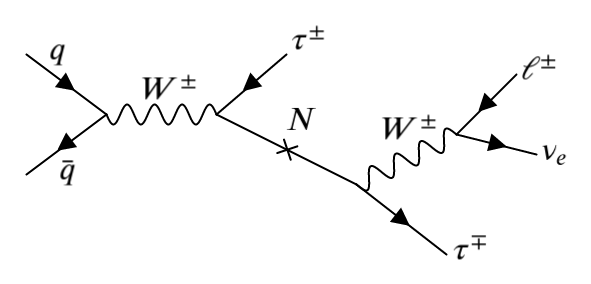
\includegraphics[width=0.7\textwidth, center]{images/RHNfeynman.png}
  \caption[RHN Feynman Diagram]{Illustrative leading order Feynman diagram for the production of RHN and its subsequent decay ($N~\rightarrow~\Wboson\tau~\rightarrow~\nu_{\ell}\ell\tau$) that may result in a multilepton final state. The taus can decay either hadronically or leptonically, giving us different channels to analyze that have different background profiles}
  \label{fig:rhnfeyn}
\end{figure}

\section{Overview}
\label{sec:overview}

The final state of an event (collision) is the set of particles seen by the detector. A lot of processes Beyond the Standard Model (BSM) produce final states with multiple leptons.  Multilepton Analysis is a useful technique for studying such processes. Since a lot of SM processes also produce multilepton final states (called background), we use this strategy to distinguish signal from background.

The model considered here [Figure~\ref{fig:rhnfeyn}] includes a right handed neutrino ($N$) that decays into a \Wboson{} boson and a $\tau$, which decay further, giving rise to multilepton final states. For this analysis, we refer to electrons and muons collectively as light leptons ($\ell$). Events are then categorized by the multiplicity of light leptons and taus ($\tau$) in these final states, into the following channels: $3\ell$, $2\ell1\tau$, $1\ell2\tau$ and $3\tau$.

To begin with, we generate the RHN acceptance cutflow table [Section~\ref{sec:cutflow}, Table~\ref{tab:cutflow}] to understand the process and how various triggers and selections affect signal acceptance. Next, we attempt to understand the process of RHN production and decay at the gen-level [Section~\ref{sec:gen}] (\ie{} from simulations). Guided by the conclusions drawn from the study of these gen-level plots, we try to carve out a signal region [Section~\ref{sec:sro}] that gives us good signal sensitivity from the phase space. Some selections used to reduce the background are explained in Section~\ref{sec:reducebkg}. We use signal significance as a metric to compare signal regions. The analysis is done for two channels: $2\ell1\tau$ and $3\ell$.

%samples
\setcounter{table}{0}
\begin{table}[t!]
  \renewcommand\thetable{1}
  \centering
  \setlength{\tabcolsep}{30pt}
  \renewcommand{\arraystretch}{2}
  \resizebox{\textwidth}{!}{%
    \begin{tabular}{c|c|c|c}
      \hline \hline
        
      \multirow{2}{*}{\textbf{Sample (RHN Mass Point)}} & \multirow{2}{*}{\textbf{Total Number of Events (n)}} &
      \multirow{2}{*}{\makecell{$\textbf{Cross-Section (xsec)}$\\
        $\textbf{(pb)}$}} &
      \multirow{2}{*}{\makecell{$\textbf{Luminosity}$\\
        $\textbf{(\ifb)}$}}\\
       & & & \\
      \hline
      \rule{0pt}{7ex}    
      100 $\GeV$ & 299,200 & 0.830 & 360.482 \\
      150 $\GeV$ & 286,200 & 0.119 & 2405.042 \\
      400 $\GeV$ & 200,000 & 0.00272 & 73529.411 \\
       & & & \\    
      \hline \hline
      
    \end{tabular}%
  }
  \caption[Data Samples]{Data samples used for this analysis. Three mass points are considered and their respective sample luminosities are calculated using the formula $L_{sample}$ = n$_{sample}$ / xsec$_{sample}$}
  \label{tab:samples}
\end{table}

\section{Object and Event Selections}
\label{sec:selections}

To better identify particles significant to our analysis, we apply certain basic preselections and triggers to the data. Object selections are listed in Table~\ref{tab:objselemu} and Table~\ref{tab:objseltau}. Triggers are listed below. A few corrections like MET filters (on data and MC both) and tau energy scale corrections are also applied.

Triggers:
\begin{itemize}
\item Leading muon $\pt>$ 26$\GeV$ 
\item Leading electron $\pt>$ 30$\GeV$ 
\item For Single Muon PD, HLT\_IsoMu24 \& HLT\_IsoTkMu24 (in data only)
\item For Single Electron PD, HLT\_Ele27\_WPTight\_Gsf (in data only)
\end{itemize}

%object sel - e/mu
\begin{table}[h!]
  \centering
  \scriptsize
  \setlength{\tabcolsep}{30pt}
  \renewcommand{\arraystretch}{2}
  \resizebox{\textwidth}{!}{%
    \begin{tabular}{c|c}
      \hline \hline
      \makecell[c]{\textbf{Muons}} & \makecell[c]{\textbf{Electrons}}\\
      \hline
       
      \makecell[l]{\\$\sbullet \hspace{0.3cm} \pt>10, |\eta|<2.4$ \\
        $\sbullet \hspace{0.2cm}$ Prompt ($d_{xy}<0.05, d_{z}<0.1$ cuts)\\
        $\sbullet \hspace{0.2cm}$ POG Medium ID\\
        $\sbullet \hspace{0.2cm}$ Relative dB-corrected isolation \\$\hspace{0.3cm}$ tight WP $(<0.15$ in $\DeltaR=0.4)$ \vspace{0.4cm}}&
      
      \makecell[l]{\\$\sbullet \hspace{0.2cm} \pt>10, |\eta|<2.5$ \\
        $\sbullet \hspace{0.2cm}$Prompt ($d_{xy}<0.05(0.1), d_{z}<0.1(0.2)$ \\ $\hspace{0.3cm}$in barrel(endcap) region)\\
        $\sbullet \hspace{0.2cm}$Cut-based Medium ID\\
        $\sbullet \hspace{0.2cm}$Relative rho-corrected isolation \\$\hspace{0.2cm}$ Medium WP (included in ID) \vspace{0.4cm}}
      \\
      \hline \hline

    \end{tabular}%
  }
  \caption{Object selections for light leptons}
  \label{tab:objselemu}
\end{table}

%object sel - tau
\begin{table}
  \centering
  \setlength{\tabcolsep}{30pt}
  \renewcommand{\arraystretch}{2}
  \resizebox{\textwidth}{!}{%
    \begin{tabular}{c|c}
      \hline \hline
      \multicolumn{2}{c}{\textbf{Taus}}\\
      \hline
      MVA ID (old) & Deep ID (new)\\
      \hline
 
      \makecell[l]{\\$\sbullet \hspace{0.3cm} \pT>20, |\eta|<2.3$ \\
        $\sbullet \hspace{0.2cm}$ Prompt ($d_{z}<0.2$ cut)\\
        $\sbullet \hspace{0.2cm}$ Old decayModeFinding, 1-prong \& 3-prong\\
        $\sbullet \hspace{0.2cm}$ '2017v2' ID\\
        $\sbullet \hspace{0.2cm}$ againstElectron \& againstMuon discriminators, loose WP\\
        $\sbullet \hspace{0.2cm}$ Cleaning against tight ID light leptons ($\DeltaR>0.4$)  \vspace{0.7cm}}  &
      
      \makecell[l]{\\$\sbullet \hspace{0.3cm} \pT>20, |\eta|<2.3$ \\
        $\sbullet \hspace{0.2cm}$ Prompt ($d_{z}<0.2$ cut)\\
        $\sbullet \hspace{0.2cm}$ New decayModeFinding, 1-prong \& 3-prong\\
        $\sbullet \hspace{0.2cm}$ Tau\_idDeepTau2017v2p1VSe $\geq 15$ \& \\ $\hspace{0.3cm}$ Tau\_idDeepTau2017v2p1VSmu $\geq 3$ (Loose WP)\\
        $\sbullet \hspace{0.2cm}$ Tau\_idDeepTau2017v2p1VSjet > 31 (Tight WP) \vspace{0.7cm}}
      \\
      \hline \hline
      
      
    \end{tabular}%
  }
  \caption[Object selections for taus]{Object selections for taus. A comparision between the two object IDs is given in Section~\ref{sec:cutflow}.}
  \label{tab:objseltau}
\end{table}

%event selection flow
\begin{wrapfigure}[10]{r}{0.15\textwidth} %the [10] is to end the wrap before the next section starts
  \scriptsize
  \centering
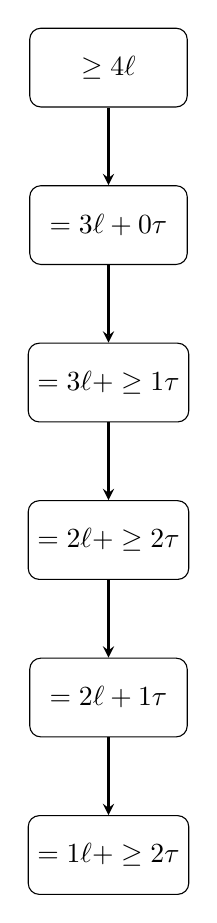
\begin{tikzpicture}[node distance = 2cm]
  \node(a)[io]{$\geq4\ell$};
  \node(b)[startstop, below of=a]{$=3\ell + 0\tau$};
  \node(c)[startstop, below of=b]{$=3\ell + \geq1\tau$};
  \node(d)[startstop, below of=c]{$=2\ell + \geq2\tau$};
  \node(e)[startstop, below of=d]{$=2\ell + 1\tau$};
  \node(f)[io, below of=e]{$=1\ell + \geq2\tau$};
  \draw[arrow] (a)--(b);
  \draw[arrow] (b)--(c);
  \draw[arrow] (c)--(d);
  \draw[arrow] (d)--(e);
  \draw[arrow] (e)--(f);
\end{tikzpicture}

\caption{Event selection flow}
\label{fig:eventselflow}
\end{wrapfigure}

The events used for analysis are selected only if they pass certain conditions (selections) listed in Table~\ref{tab:eventsel}. An event is selected for a channel only if it fails the selections for all the previous channels. The order of priority (event selection flow) is illustrated in Figure~\ref{fig:eventselflow}.

%event sel
\begin{table}
  \centering
  \setlength{\tabcolsep}{30pt}
  \renewcommand{\arraystretch}{1.2}
  \resizebox{\textwidth}{!}{%
  \begin{tabular}{l}
    \hline \hline
    \centerline{\textbf{Event Selections}}\\
    \hline
    \centerline{$3\ell$}\\
    \hline
    $\sbullet \hspace{0.2cm}$ Leading light lepton ($e/\mu$) passing triggers\\
    $\sbullet \hspace{0.2cm}$ Altleast two more light leptons ($e/\mu$), $\pt>10,10 \GeV$\\
    $\sbullet \hspace{0.2cm}$ Minimum invariant mass of same flavor (SF) light lepton pair $> 12 \GeV$\\
    $\sbullet \hspace{0.2cm}$ Minimum $\DeltaR$ between all leptons in the event $> 0.4$\\
    $\sbullet \hspace{0.2cm}$ Triggers (in data only)\\
    \hline
    \centerline{$2\ell1\tau$}\\
    \hline
    $\sbullet \hspace{0.2cm}$ Event should fail $3\ell$ selection\\
    $\sbullet \hspace{0.2cm}$ Leading light lepton ($e/\mu$) passing triggers\\
    $\sbullet \hspace{0.2cm}$ Another light lepton ($e/\mu$), $\pt>10 GeV$\\
    $\sbullet \hspace{0.2cm}$ Minimum invariant mass of same flavor (SF) light lepton pair $> 12 \GeV$\\
    $\sbullet \hspace{0.2cm}$ Atleast one hadronic tau, $\pt>20 \GeV$\\
    $\sbullet \hspace{0.2cm}$ $\DeltaR>0.4$ among the three leptons\\
    $\sbullet \hspace{0.2cm}$ Triggers (in data only)\\
    \hline
    \centerline{$1\ell2\tau$}\\
    \hline
    $\sbullet \hspace{0.2cm}$ Exactly one light lepton ($e/\mu$), for triggering\\
    $\sbullet \hspace{0.2cm}$ Atleast two hadronic taus, $\pt>20,20 \GeV$\\
    \hspace{1cm}- Prompt taus pass tight ID, fake taus pass loose ID\\
    $\sbullet \hspace{0.2cm}$ $\DeltaR>0.4$ among the three leptons\\
    $\sbullet \hspace{0.2cm}$ Triggers (in data only)\\
    $\sbullet \hspace{0.2cm}$ Event should fail all other event ($3\ell,2\ell+\geq1\tau..$) selections\\
    \hline \hline
    \end{tabular}%
  }
  \caption{Event selections for 3$\ell$, 2$\ell$1$\tau$ and 1$\ell$2$\tau$ channels}
  \label{tab:eventsel}
\end{table}

\section{Background}
\label{sec:bkgs}

%bkgs feynman diagrams
\begin{figure}
  \begin{adjustbox}{minipage=\textwidth, scale=0.75}
    \centering
    \subfloat[DY]{{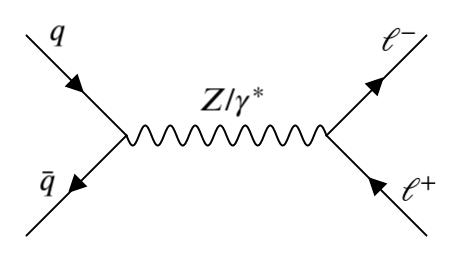
\includegraphics[width=0.3\textwidth]{images/DYfeynman.png} }}%
    \qquad
    \subfloat[\ttbar]{{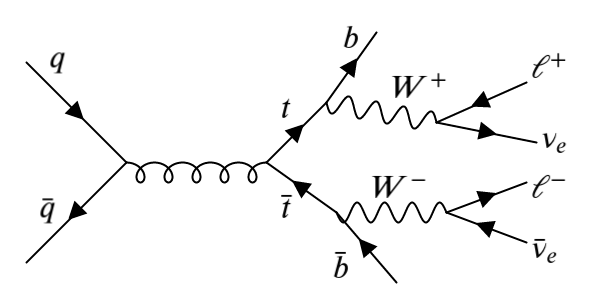
\includegraphics[width=0.3\textwidth]{images/ttbarfeynman.png} }}%
    \caption[Feynman diagrams for background processes]{\normalsize{Leading order Feynman diagrams for fake background processes. \emph{(a)} The Drell-Yan process. The third lepton can be faked by another particle/jet. \emph{(b)} One of the possible decay products of the \ttbar{} process}}
    \label{fig:bkgsfeyn}
  \end{adjustbox}
\end{figure}
Many SM processes give rise to multilepton final states, and our objective is to distinguish these processes (background) from the signal (RHN). The method used for background estimation in this analysis is Monte-Carlo based. All the background processes considered are listed in Table~\ref{tab:bkgs}. \WZ{} and \ZZ{} are prompt backgrounds while DY and \ttbar{} are fake (\ie{} one of the leptons is faked by another particle/jet).   


%bkgs
\begin{table}
  \centering
  \setlength{\tabcolsep}{30pt}
  \renewcommand{\arraystretch}{1.9}
  \resizebox{\textwidth}{!}{%
    \begin{tabular}{p{0.0001\textwidth}|p{0.15\textwidth}|c|c|c}
      \hline \hline
      \multicolumn{2}{c|}{\multirow{2}{*}{\textbf{Background}}} &
      \multirow{2}{*}{\textbf{Total Number of Events (n)}} &
      \multirow{2}{*}{\makecell{$\textbf{Cross-Section (xsec)}$\\
        $\textbf{(pb)}$}} &
      \multirow{2}{*}{\makecell{$\textbf{Luminosity}$\\
        $\textbf{(\ifb)}$}}\\
      \multicolumn{2}{c|}{} & & & \\
      \hline
      \multirow{4}{*}{\begin{sideways} {\large{$2\ell1\tau$}} \end{sideways}} & DY & 89,832,690 & 5765 & 15.582\\
      & $\WZ$ & 6,610,401 & 5.052 & 1308.472\\
      & $\ZZ$ & 7,547,891 & 1.325 & 5696.521\\
      & $\ttbar$ & 24,265,024 & 88.29 & 274.833\\   
      \hline
      \multirow{4}{*}{\begin{sideways} {\large{$3\ell$}} \end{sideways}} & DY & 89,832,690 & 5765 & 15.582\\
      & $\WZ$ & 1,295,229 & 5.052 & 256.378\\
      & $\ZZ$ & 1,041,601 & 1.325 & 786.114\\
      & $\ttbar$ & 24,265,024 & 88.29 & 274.833\\   
     \hline \hline
    \end{tabular}%
  }
  \caption[Backgrounds]{A few background processes and their luminosities. Luminosity is calculated by the formula $L$~=~n~/~xsec}
  \label{tab:bkgs} 
\end{table}


\section{Signal Region Optimization}
\label{sec:sro}


The objective of Signal Region optimization is to find a region in the phase space in which the signal is easily distinguished from background. A metric for the same is signal significance, defined as-
\[
\textrm{Significance} = \frac{\textrm{Signal}}{\sqrt{\textrm{Background}}}
\]

The higher the significance, the better is the signal region. We perform signal region optimization for the $2\ell1\tau$ and $3\ell$ channels separately because the background profiles for these channels are different.

\subsection{Understanding the Process with Simulations}
\label{sec:gen}

To undrestand the general topology of the events, like the \DeltaR{} $=\sqrt{(\Delta \eta)^{2} + (\dphi)^{2}}$\enskip between leptons and the origin (mother particle) of the particles involved, we plot these quantities using simulated data.
\vspace{0.7cm}
\begin{figure}[h]
\centering
\subfloat[{\scriptsize RHN \pT{} [\GeV]}]{{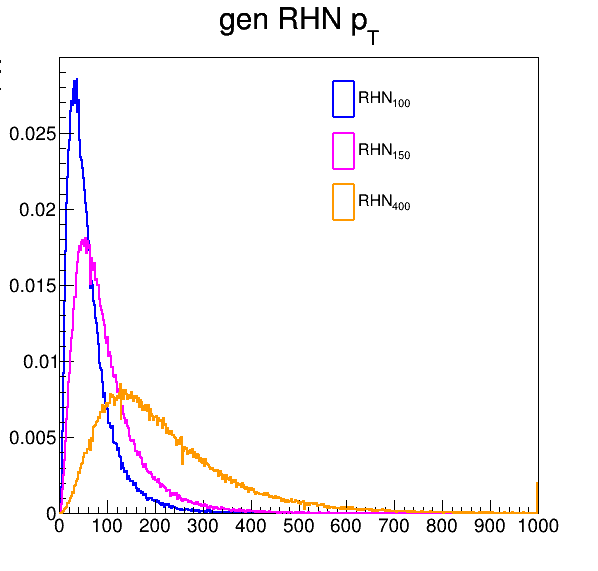
\includegraphics[trim=10 0 0 50,clip, width=0.3\textwidth]{images/RHN_pT.png} }}%
\qquad
\subfloat[{\scriptsize PDG-ID of RHN Mothers}]{{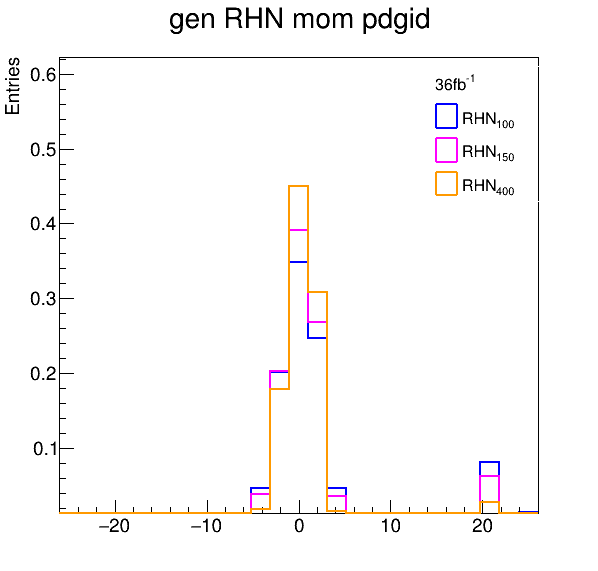
\includegraphics[trim=30 0 0 50,clip, width=0.29\textwidth]{images/RHN_momid.png} }}%
\qquad
\subfloat[{\scriptsize\pT{} of $\tau$ coming from PV [\GeV] }]{{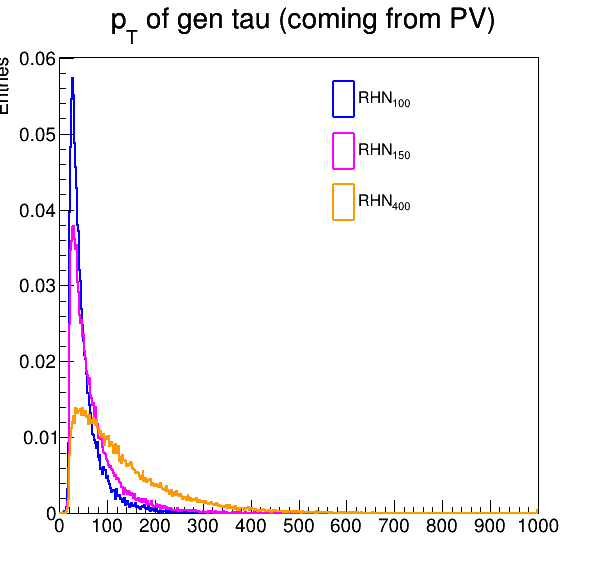
\includegraphics[trim=10 0 0 50,clip, width=0.3\textwidth]{images/pvtaupt.png} }}%
\qquad
\subfloat[{\scriptsize \DeltaR{} (RHN,$\tau$)}]{{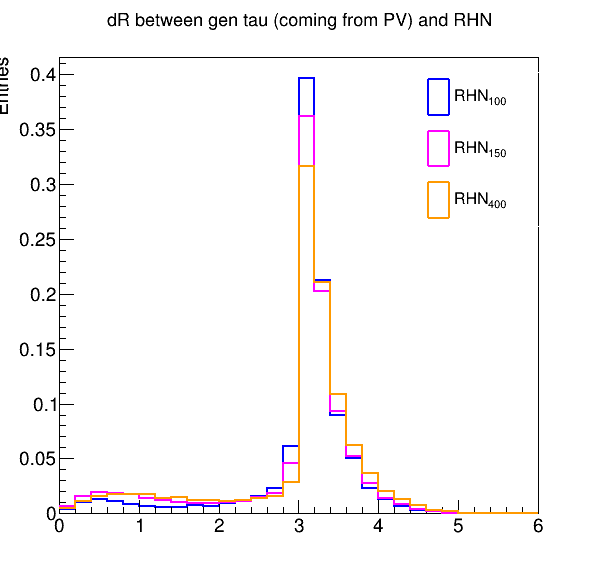
\includegraphics[trim=10 0 0 50,clip, width=0.3\textwidth]{images/pvtaudRRHN.png} }}%
\caption[RHN gen plots]{Gen plots for the production of RHN (all the plots have been normalized to unity). \emph{(a)} Transverse momenta of RHN of different mass points. We can see that the 400\GeV{} RHN (yellow) is more boosted than the 100\GeV{} RHN (blue). \emph{(b)} PDG-ID of mother particles of RHN. We observe that they are mostly quarks. \emph{(c)} Transverse momentum of the $\tau$ coming from the production vertex (PV). \emph{(d)} \DeltaR{} between RHN and $\tau$ coming from PV. We observe that they are produced back-to-back.}

\label{fig:gen}  
\end{figure}
\clearpage

Next, we look at the final state leptons and their plots. Here, we divide the $2\ell1\tau$ channel further into two categories: (1) OS (opposite-sign) in which the two light leptons have opposite signs and (2) SS (same-sign) in which they have the same sign. The motivation behind this is that these two categories will have different dominating backgrounds. For instance, the $2\ell1\tau$-OS category is likely to have DY in large numbers because DY cannot produce same-sign dileptons.

\vspace{0.7cm}
\begin{figure}[h]
\centering
\subfloat[{\scriptsize $\ell_{1}$ Mother PDG-ID}]{{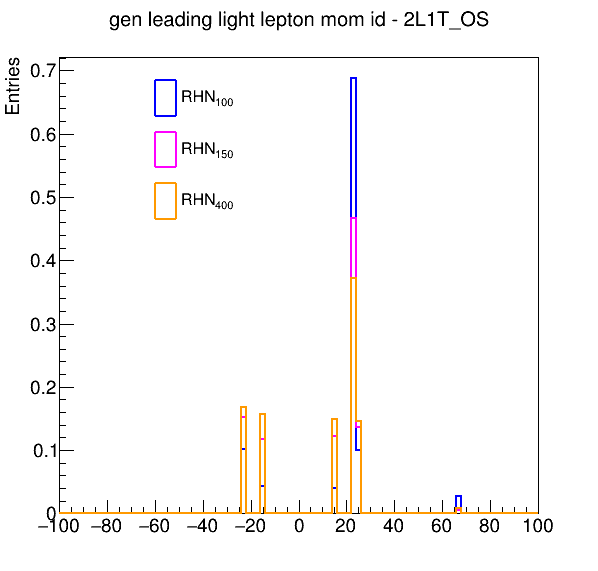
\includegraphics[trim=0 0 0 50,clip, width=0.3\textwidth]{images/2L1T_OS_momidL1.png} }}%
\quad
\subfloat[{\scriptsize $\ell_{2}$ Mother PDG-ID}]{{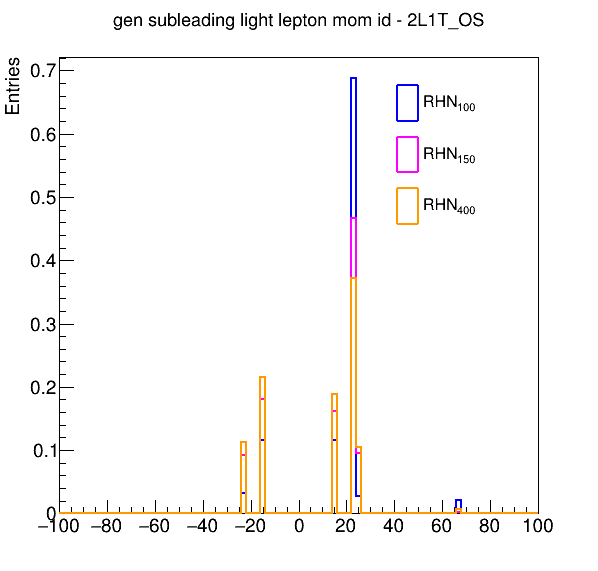
\includegraphics[trim=0 0 0 50,clip, width=0.3\textwidth]{images/2L1T_OS_momidL2.png} }}%
\quad
\subfloat[{\scriptsize $\tau$ Mother PDG-ID }]{{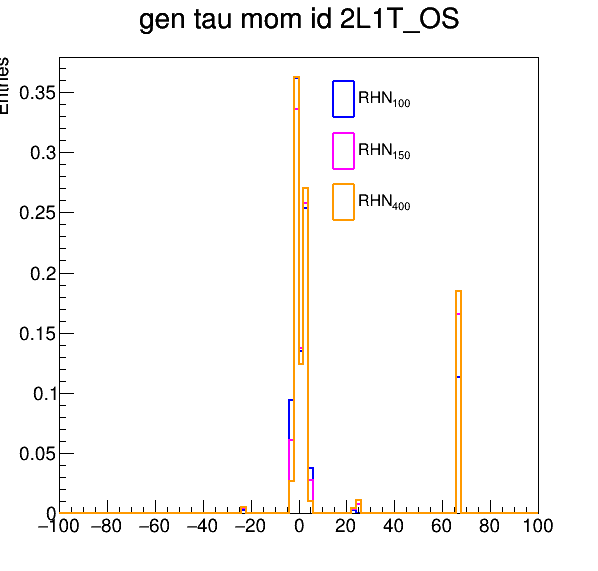
\includegraphics[trim=0 0 0 50,clip, width=0.3\textwidth]{images/2L1T_OS_momidT.png} }}%
\quad

\caption[Gen plots for \2l1t-OS]{Gen plots for the $2\ell1\tau$-OS channel (all the plots have been normalized to unity). All the entries for RHN have been made at ID = 66 (instead of 9900012). \emph{(a)} PDG-ID of the mother of the leading light lepton $\ell_{1}$. We see peaks at $\pm15$ and $\pm24$ which correspond to taus and \Wboson{} bosons respectively. \emph{(b)} PDG-ID of the mother of the sub-leading light lepton $\ell_{2}$. \emph{(c)} PDG-ID of the mother of the $\tau$. We see peaks at 66 and within the range (-6,6), which correspond to RHN and quarks respectively.}

\label{fig:2l1tOSgen}  
\end{figure}

\vspace{0.7cm}

When we compare Figure~\ref{fig:2l1tOSgen} to the feynman diagram in Figure~\ref{fig:2l1tgenfeyn} (a), we see that the observations match. From the diagram, we can further hypothesize that the light lepton pair should be close together (when boosted). Similarly, the observations from Figure~\ref{fig:2l1tSSgen} (SS gen plots) match with the ones from the Feynman diagram [Figure~\ref{fig:2l1tgenfeyn} (b)].

%gen feynman diagrams
\begin{figure}[h]
  \centering
  \subfloat[OS]{{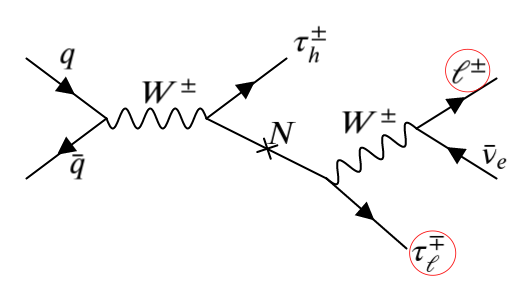
\includegraphics[width=0.4\textwidth]{images/2l1tOSfeynman.png} }}%
  \qquad
  \subfloat[SS]{{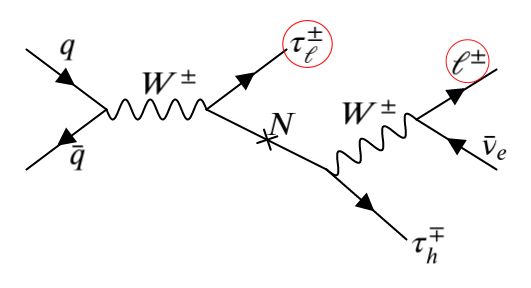
\includegraphics[width=0.4\textwidth]{images/2l1tSSfeynman.png} }}%
  \caption[Feynman diagrams for \2l1t-OS and SS]{Feynman diagrams for $2\ell1\tau$ OS and SS channels. \emph{(a)} The PV $\tau$ decays hadronically and the $\tau$ coming from the RHN decays leptonically. Since RHN is electrically neutral, the light lepton pair in the final state will be OS in this case. \emph{(b)} The only way an SS pair can be produced is for one of the light leptons to be a product of the PV $\tau$ decay, since the daughters of RHN will have to be OS (note that this can result in an OS pair as well).}
  \label{fig:2l1tgenfeyn}
\end{figure}

\clearpage

\begin{figure}[h]
\centering
\subfloat[{\scriptsize $\ell_{1}$ Mother PDG-ID}]{{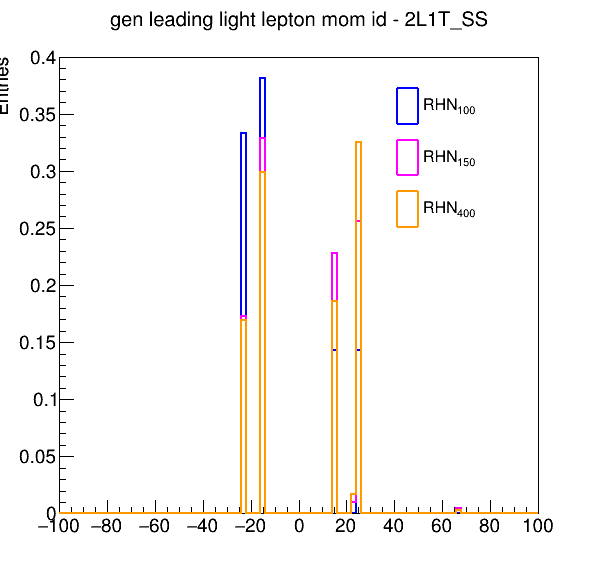
\includegraphics[trim=0 0 0 50,clip, width=0.3\textwidth]{images/2L1T_SS_momidL1.png} }}%
\quad
\subfloat[{\scriptsize $\ell_{2}$ Mother PDG-ID}]{{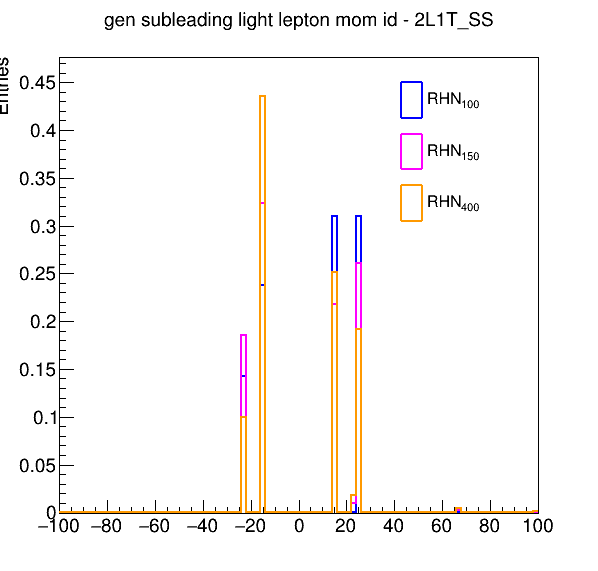
\includegraphics[trim=0 0 0 50,clip, width=0.3\textwidth]{images/2L1T_SS_momidL1L2.png} }}%
\quad
\subfloat[{\scriptsize $\tau$ Mother PDG-ID }]{{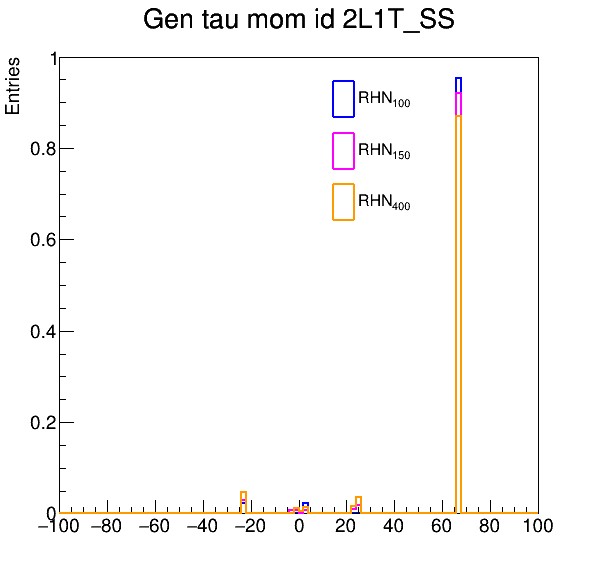
\includegraphics[trim=0 0 0 50,clip, width=0.3\textwidth]{images/2L1T_SS_momidT.png} }}%
\quad

\caption[Gen plots for \2l1t-SS]{Gen plots for the $2\ell1\tau$-SS channel (all the plots have been normalized to unity). All the entries for RHN have been made at ID = 66 (instead of 9900012). \emph{(a)} PDG-ID of the mother of the leading light lepton $\ell_{1}$. Again, we see peaks at taus and \Wboson{} bosons, but this time the peak at $\tau$ is comparable to the one at \Wboson{} boson. \emph{(b)} PDG-ID of the mother of the sub-leading light lepton $\ell_{2}$. \emph{(c)} PDG-ID of the mother of the $\tau$. We see a peak only at RHN.}
\label{fig:2l1tSSgen}  
\end{figure}

In conclusion, we decide to divide the $2\ell1\tau$ channel into OS and SS categories, owing to the differences in their production and backgrounds. For a better understanding, we study the $1\ell2\tau$ channel in a similar manner [Figure~\ref{fig:1l2tgen}]. We observe that the PV $\tau$ is almost always the leading $\tau$.

\vspace{0.7cm}
\begin{figure}[h]
\centering
\subfloat[{\scriptsize $\tau_{1}$ Mother PDG-ID}]{{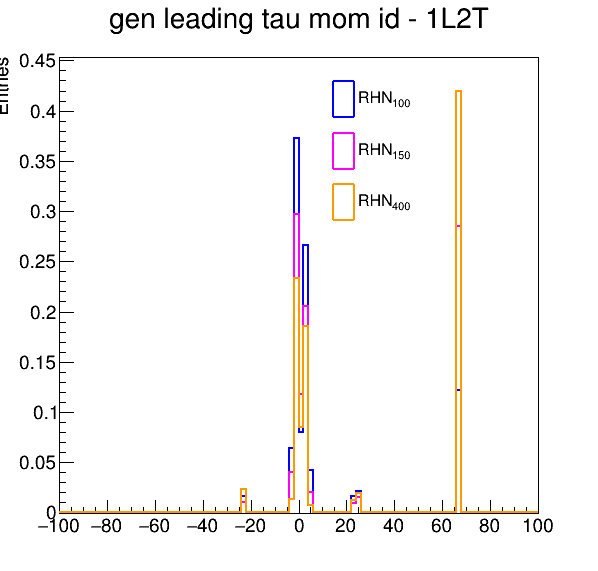
\includegraphics[trim=0 0 0 50,clip, width=0.3\textwidth]{images/1L2T_momidT1.png} }}%
\quad
\subfloat[{\scriptsize $\tau_{2}$ Mother PDG-ID}]{{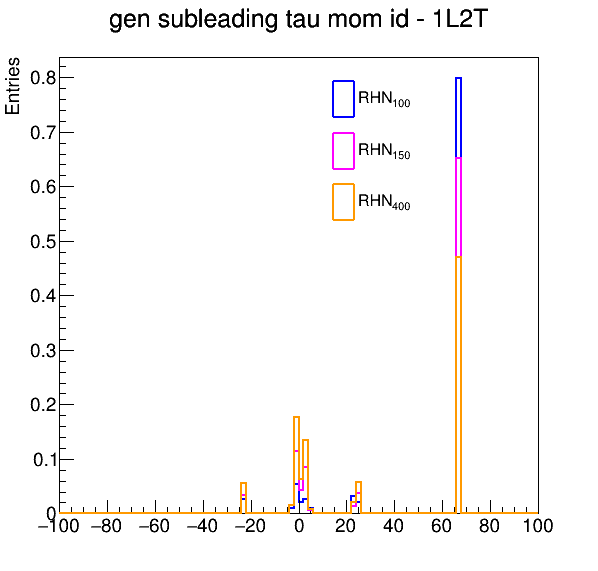
\includegraphics[trim=0 0 0 50,clip, width=0.3\textwidth]{images/1L2T_momidT2.png} }}%
\quad
\subfloat[{\scriptsize $\ell$ Mother PDG-ID }]{{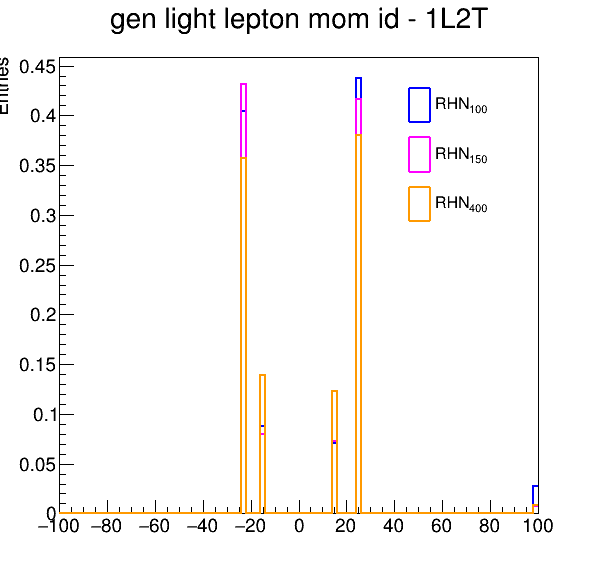
\includegraphics[trim=0 0 0 50,clip, width=0.3\textwidth]{images/1L2T_momidL.png} }}%
\quad

\caption[Gen plots for \1l2t]{Gen plots for the $1\ell2\tau$ channel (all the plots have been normalized to unity). All the entries for RHN have been made at ID = 66 (instead of 9900012). \emph{(a)} PDG-ID of the mother of the leading tau $\tau_{1}$. We see peaks at RHN and quarks. \emph{(b)} PDG-ID of the mother of the sub-leading tau $\tau_{2}$. \emph{(c)} PDG-ID of the mother of the light lepton $\ell$.}
\label{fig:1l2tgen}  
\end{figure}

\subsection{Reducing Background}
\label{sec:reducebkg}

Based on our understanding of the SM background processes and the RHN decay, we can apply specific selections to kill the background to a large extent. The following conditions or vetoes were applied:

\begin{enumerate}
  \item \textbf{On-\boldmath{\Zboson} veto}: In the process of RHN decay, the light leptons are daughters of \Wboson{} bosons or $\tau$. In the background processes (like \ZZ, \WZ{} and DY), many of the light leptons are daughters of the \Zboson{} boson. Thus, we exclude the on-\Zboson{} region, \ie{} we exculde events for which the invariant mass of the light lepton pair ($M_{\ell_{1}\ell_{2}}$) is in the on-\Zboson{} range. We define this range to be $76\GeV - 106\GeV$ (\Zboson-mass is $91\GeV$). Table~\ref{tab:reducebkg} and Figure~\ref{fig:reducebkg} show how this veto affects the background and signal.

\begin{table}[h]
  \centering
  \footnotesize
  \setlength{\tabcolsep}{20pt}
  \renewcommand{\arraystretch}{1.6}
  \resizebox{0.6\textwidth}{!}{%
    \begin{tabular}{c|l|r|r}
    \hline \hline
    & Region & Events Before Veto & Events After Veto\\
    \hline
\multirow{3}{*}{DY} & $2\ell1\tau$ & $10,512$ & $745$\\
& $2\ell1\tau$-OS & $10,456$ & $738$\\
& $2\ell1\tau$-SS & $56$ & $7$\\
\hline
\multirow{3}{*}{\ttbar} & $2\ell1\tau$ & $3,719$ & $1,046$\\
& $2\ell1\tau$-OS & $3,377$ & $942$\\
& $2\ell1\tau$-SS & $342$ & $104$\\
\hline
\multirow{3}{*}{M100} & $2\ell1\tau$ & $413$ & $154$\\
& $2\ell1\tau$-OS & $371$ & $125$\\
& $2\ell1\tau$-SS & $42$ & $27$\\
\hline
\multirow{3}{*}{M150} & $2\ell1\tau$ & $2,560$ & $1,199$\\
& $2\ell1\tau$-OS & $2,161$ & $880$\\
& $2\ell1\tau$-SS & $390$ & $305$\\
\hline \hline
    \end{tabular}%
    }
  \caption[Effect of on-\Zboson{} veto]{The number of events before and after applying the On-\Zboson{} veto. The signal also reduces with the background but the overall significance improves in every region.}
  \label{tab:reducebkg}
\end{table}

\vspace{0.5cm}
\begin{figure}[h]
  \centering
\subfloat[{\scriptsize \Lt{} before On-\Zboson{} veto [\GeV]}]{{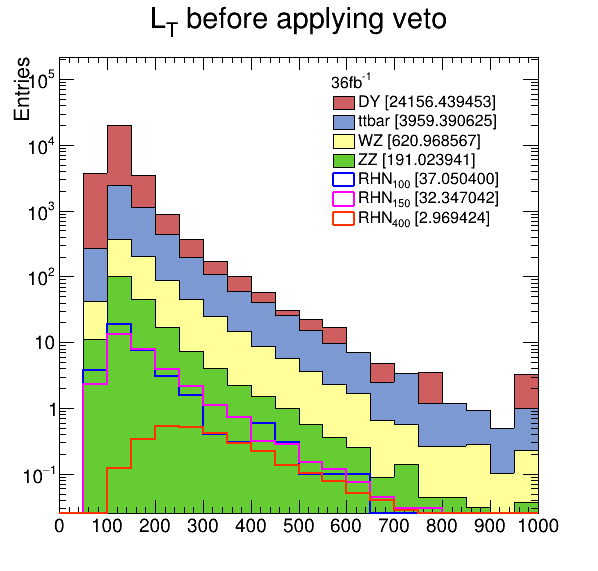
\includegraphics[trim=0 0 0 40,clip, width=0.45\textwidth]{images/Ltbv.png} }}%
\qquad
\subfloat[{\scriptsize \Lt{} after On-\Zboson{} veto [\GeV]}]{{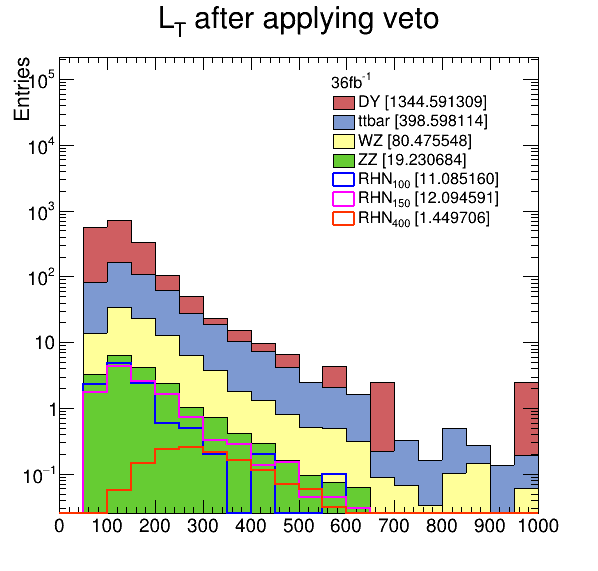
\includegraphics[trim=0 0 0 40,clip, width=0.45\textwidth]{images/Ltav.png} }}%

\caption[Effect of on-\Zboson{} veto]{\Lt{} plots before and after the application of the On-\Zboson{} veto (\Lt{} is defined as the scalar sum of the \pt{} for the final state leptons). All the sample luminosities have been scaled to the integrated luminosity of $36$ \ifb{} so that the comparision is accurate.}
\label{fig:reducebkg}  
\end{figure}

\item \textbf{\boldmath$N_{Bjets}$ veto}: This veto is majorly for cutting down \ttbar{} background. The \ttbar{} decay produces b-jets [Figure~\ref{fig:bkgsfeyn}] while RHN does not. So, we include events which have no b-jets ($N_{Bjets}~=~0$).

  \item \textbf{\boldmath$H_{T}^{50} < 100$ veto}: RHN decay usually does not result in high energy jets, while other background processes might. So we put a upper limit on the sum of \pt{} of all jets in an event. This variable is named $H_{T}$. We use a modified variable $H_{T}^{50}$ which puts a lower limit of $50$ on jet \pt. This is to avoid pileup and consider real jets only.
  \end{enumerate}

  
\subsection{\Large{\boldmath$2\ell1\tau$}}
\label{sec:2l1t}

Guided by the observations and conclusions from the gen plots, and after applying vetoes to kill background, we try to find a region with appropriate selections. To begin, we study some basic plots:

%metpt
\vspace{0.5cm}
\begin{figure}[h]
  \centering
  \subfloat[{\scriptsize \metpt{} (\2l1t-OS) [\GeV]}]{{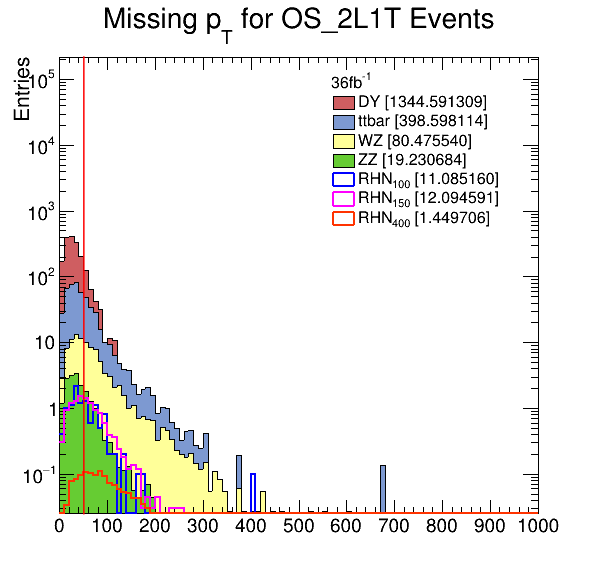
\includegraphics[trim=0 0 0 40,clip, width=0.45\textwidth]{images/metpt.png} }}%
  \qquad
  \subfloat[{\scriptsize \metpt{} (\2l1t-SS) [\GeV]}]{{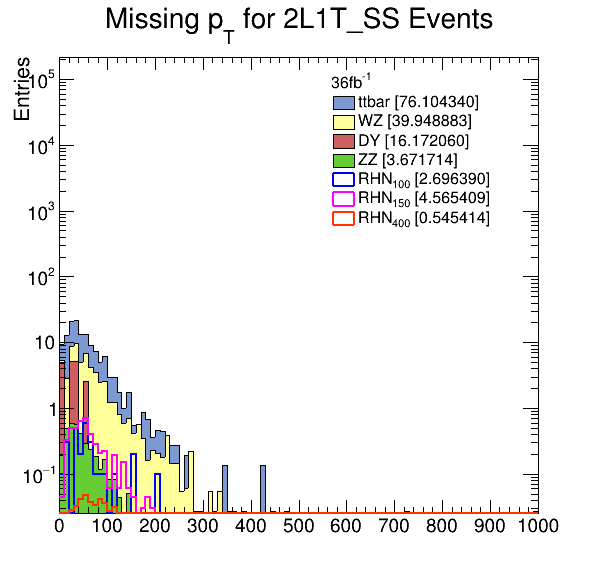
\includegraphics[trim=0 0 0 45,clip, width=0.45\textwidth]{images/metpt-ss.png} }}%
  \vspace{0.6cm}
  \tiny
  \setlength{\tabcolsep}{20pt}
  \renewcommand{\arraystretch}{1.6}
  \begin{tabular}{|c|c|c|}
    \hline
    \2l1t-OS & \2l1t-OS \metpt $<50$ & \2l1t-OS \metpt $>50$\\
    \hline
    \Gape[0.2cm]{\makecell{
        \sig{} $(100) = 0.2582$\\
        \sig{} $(150) = 0.2817$\\
        \sig{} $(400) = 0.0337$ }} & 
    \makecell{
      \sig{} $(100) = 0.1564$\\
      \sig{} $(150) = 0.1399$\\
      \sig{} $(400) = 0.0079$} &
    \makecell{
      \sig{} $(100) = 0.2877$\\
      \sig{} $(150) = 0.3789$\\
      \sig{} $(400) = 0.0633$}\\
    \hline
  \end{tabular}
  
  \caption[\metpt{} for \2l1t-OS and \2l1t-SS]{\metpt{} for \2l1t OS and SS channels. In \emph{(a)}, we observe that most of the DY background lies in the low \metpt{} range. This is confirmed by the significance table. Thus, \metpt $>50$ will be our first selection, \ie{} we exculde the region below $50\GeV$.}
  \label{fig:2l1tmetpt}
\end{figure}

\subsubsection{{\Large{\boldmath$2\ell1\tau$}} - OS}
\label{sec:2l1tOS}

After studying the \metpt{} plots for the OS channel [Figure~\ref{fig:2l1tmetpt}], we decide to select the region in which \metpt{} is above $50$. This eliminates a lot of DY background. All the following plots are of the \metpt{} $>50$ region. In Figure~\ref{fig:2l1tOSplots}, we have the \pt{} and \DeltaR{} plots. We observe that the light lepton pair for RHN events is generally closer together [Fig.~\ref{fig:2l1tOSplots}\emph{(d)}] and that the sub-leading light lepton and the tau are far apart [Fig.~\ref{fig:2l1tOSplots}\emph{(f)}](as expected from simulations).

Next, we plot a number of physical quatities like \dphi, $m_{\ll\ls}$, transverse mass ($m_{T}$), visible transverse mass, etc. We also define a few new variables like \MET/$m_{T}$ and $m_{T}$ ($\ell_{res}$, \MET) where $\ell_{res}$ is defined as the vector sum of one of the two OS pairs. Transverse mass is defined as -

\[
m_{T} = \sqrt{2\pt^{miss}\pt^{\ell}[1 - cos(\dphi_{m_{T}})]}
\]

where $\pt^{\ell}$ is the \pt{} of the lepton under consideration.

%OS plots
\begin{figure}[h!]
  \centering
  \makebox[0pt][c]{%
  \subfloat[{\scriptsize \pt{} of leading light lepton \ll [\GeV]}]{{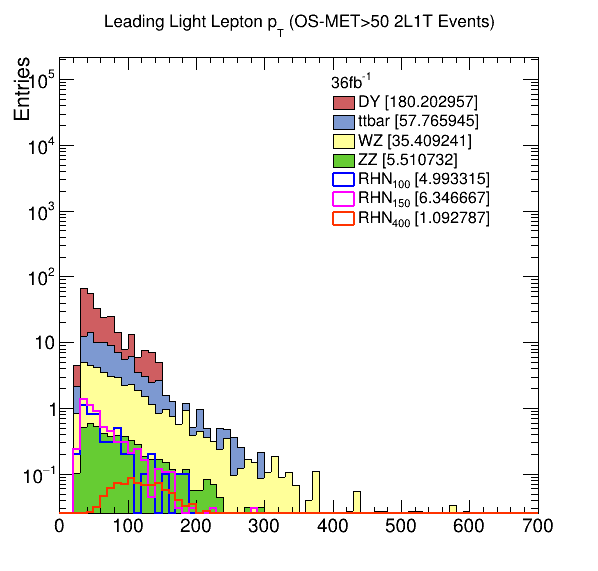
\includegraphics[trim=0 0 0 45,clip, width=0.35\textwidth]{images/llpt.png}}}
  \enskip
  \subfloat[{\scriptsize \pt{} of sub-leading light lepton \ls [\GeV]}]{{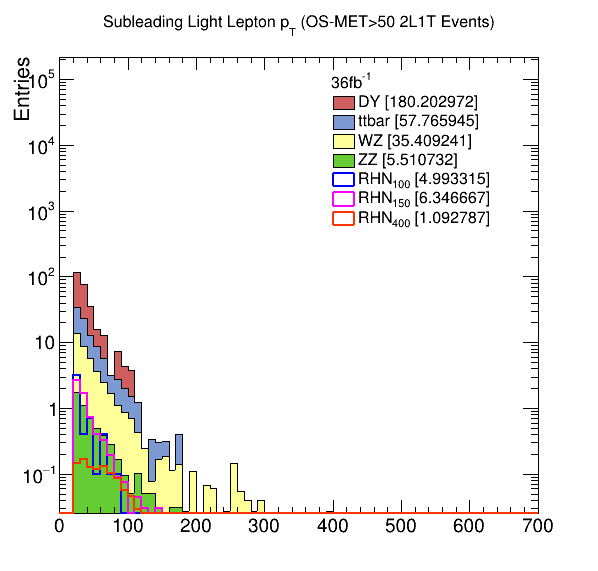
\includegraphics[trim=0 0 0 45,clip, width=0.35\textwidth]{images/slpt.png} }}%
  \enskip
  \subfloat[{\scriptsize \pt{} of $\tau$ [\GeV]}]{{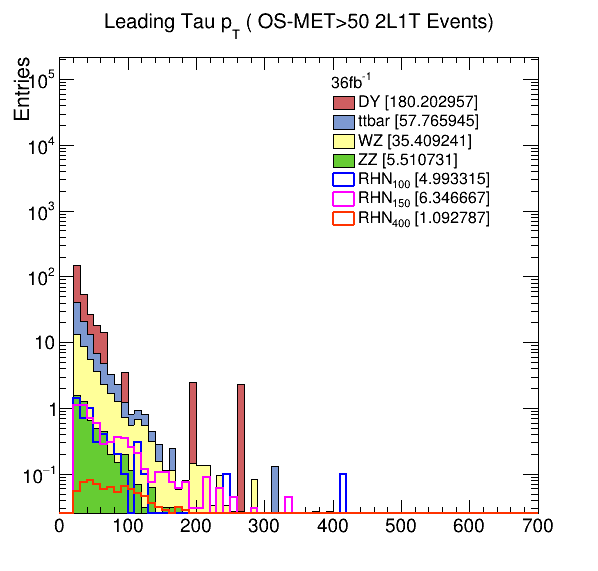
\includegraphics[trim=0 0 0 45,clip, width=0.35\textwidth]{images/tpt.png} }}%
  }
  \makebox[\textwidth][c]{%
    \rule{0pt}{0.4cm}
    }
  \makebox[0pt][c]{%
  \subfloat[{\scriptsize \DeltaR{} (\ll,\ls)}]{{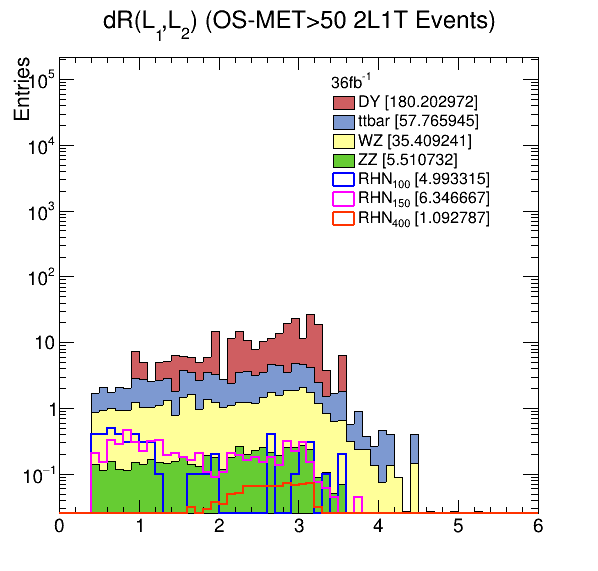
\includegraphics[trim=0 0 0 45,clip, width=0.35\textwidth]{images/dR0.png} }}%
  \enskip
  \subfloat[{\scriptsize \DeltaR{} (\ll,$\tau$)}]{{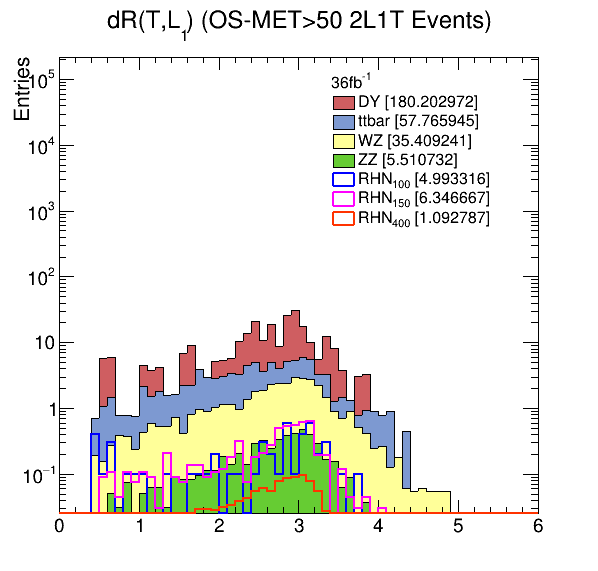
\includegraphics[trim=0 0 0 45,clip, width=0.35\textwidth]{images/dR1.png} }}%
  \enskip
  \subfloat[{\scriptsize \DeltaR{} (\ls,$\tau$)}]{{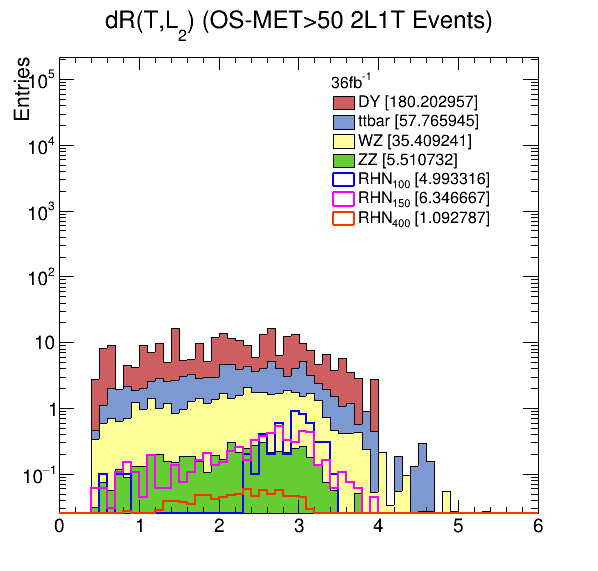
\includegraphics[trim=0 0 0 45,clip, width=0.35\textwidth]{images/dR2.png} }}%
  }
  \makebox[\textwidth][c]{%
    \rule{0pt}{0.4cm}
    }
  \makebox[0pt][c]{%
    \subfloat[{\scriptsize \Lt{} [\GeV]}]{{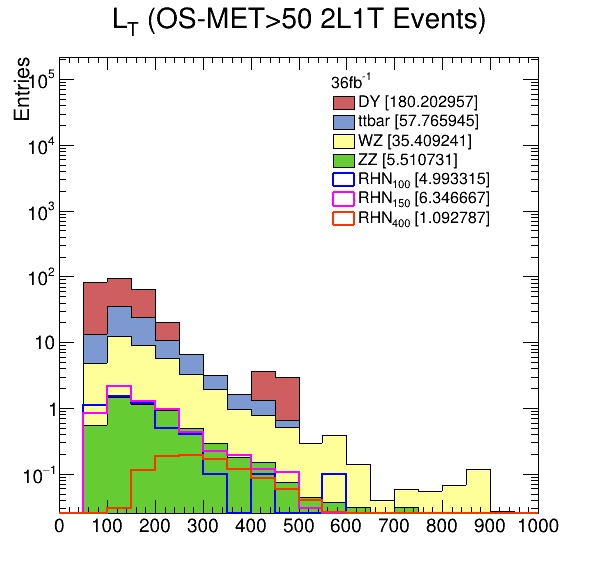
\includegraphics[trim=0 0 0 45,clip, width=0.45\textwidth]{images/Lt.png}}}
    \qquad
    \subfloat[{\scriptsize $m_{T}$ ($\tau$, \met) [\GeV]}]{{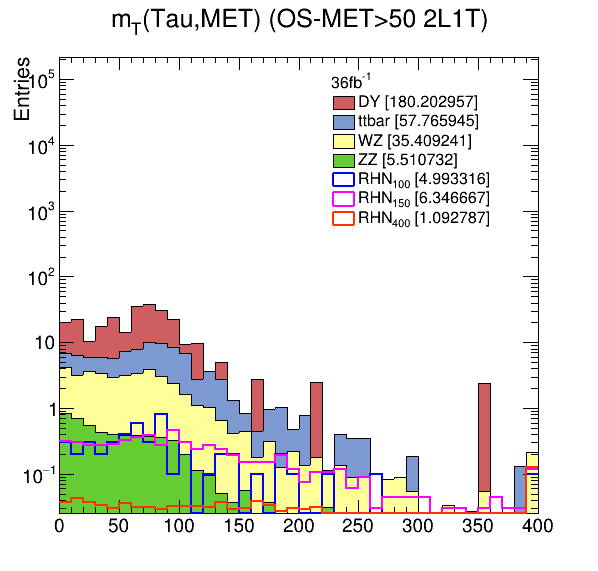
\includegraphics[trim=0 0 0 45,clip, width=0.45\textwidth]{images/mt2.png} }}%
  }
  \caption{Some basic distributions for the \2l1t-OS \metpt $>50$ region.}
  \label{fig:2l1tOSplots}
\end{figure}

Based on these plots, we attempt to find the optimal signal region so that signal significance is maximized. We try a bunch of selections (or cuts) for the same. The ones that yield the best results are given in Figures~\ref{fig:2l1tc1} to \ref{fig:2l1tc5} (\Lt{} is used as the discriminating variable). A summary of all the selections is given in Table~\ref{tab:2l1t}.

%cut 1
\begin{figure}[h!]
  \centering
  \subfloat[{\scriptsize \DeltaR{} (\ll, \ls)}]{{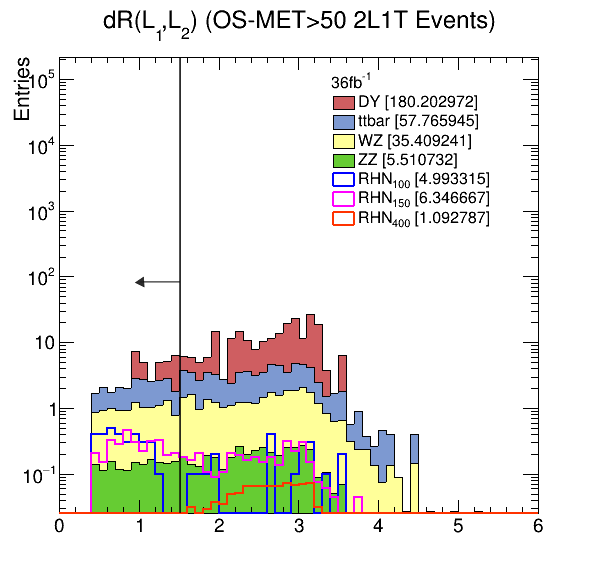
\includegraphics[trim=0 0 0 40,clip, width=0.45\textwidth]{images/2l1tc1.png} }}%
  \subfloat{{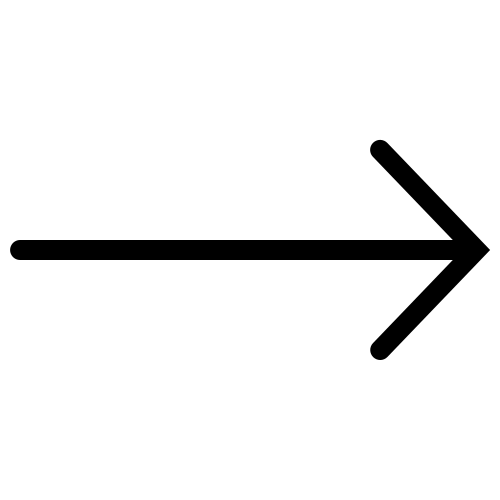
\includegraphics[trim=0 -1400 0 -1400,clip, height=7cm, width=0.1\textwidth]{images/right-arrow.png} }}%
  \subfloat[{\scriptsize \Lt{} [\GeV]}]{{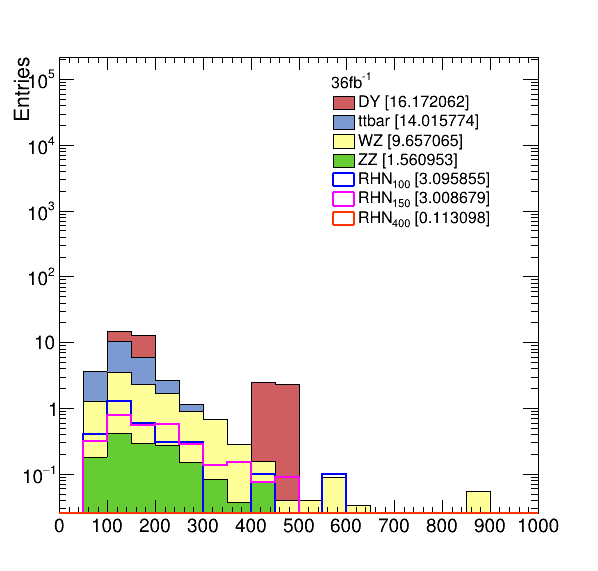
\includegraphics[trim=0 0 0 45,clip, width=0.45\textwidth]{images/2l1tc1lt.png} }}%
  \vspace{0.6cm}
  \tiny
  \setlength{\tabcolsep}{20pt}
  \renewcommand{\arraystretch}{1.6}
  \begin{tabular}{|c|c|}
    \hline
    Significance before cut & Significance after cut\\
    \hline
    \Gape[0.2cm]{\makecell{
        \sig{} $(100) = 0.2990$\\
        \sig{} $(150) = 0.3800$\\
        \sig{} $(400) = 0.0654$ }} & 
    \makecell{
      \sig{} $(100) = 0.4811$\\
      \sig{} $(150) = 0.4675$\\
      \sig{} $(400) = 0.0176$}\\
    \hline
  \end{tabular}
  \caption[\2l1t-OS Cut-1: \DeltaR{} (\ll, \ls) < 1.5]{\DeltaR{} (\ll, \ls) < 1.5 for \2l1t-OS \metpt $>50$ events.}
  \label{fig:2l1tc1}
  \vspace{1cm}
\end{figure}

%cut 2
\begin{figure}[h!]
  \centering
  \subfloat[{\scriptsize \dphi{} (\ll, \ls)}]{{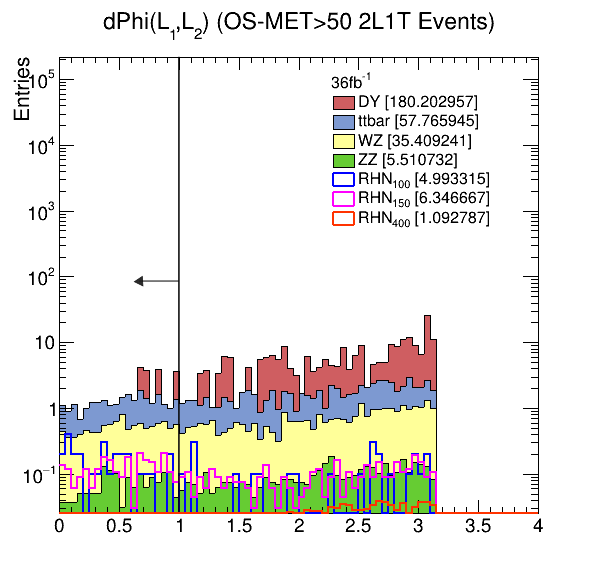
\includegraphics[trim=0 0 0 40,clip, width=0.45\textwidth]{images/2l1tc2.png} }}%
  \subfloat{{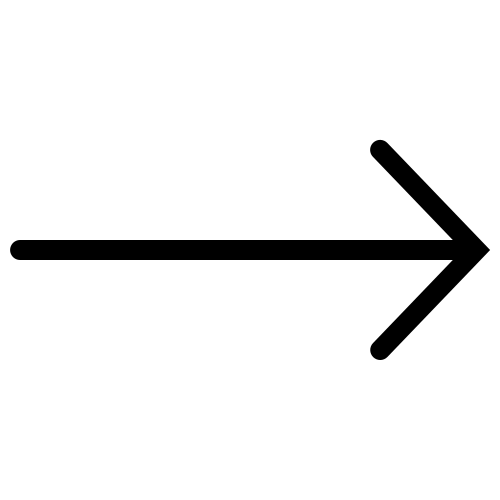
\includegraphics[trim=0 -1400 0 -1400,clip, height=7cm, width=0.1\textwidth]{images/right-arrow.png} }}%
  \subfloat[{\scriptsize \Lt{} [\GeV]}]{{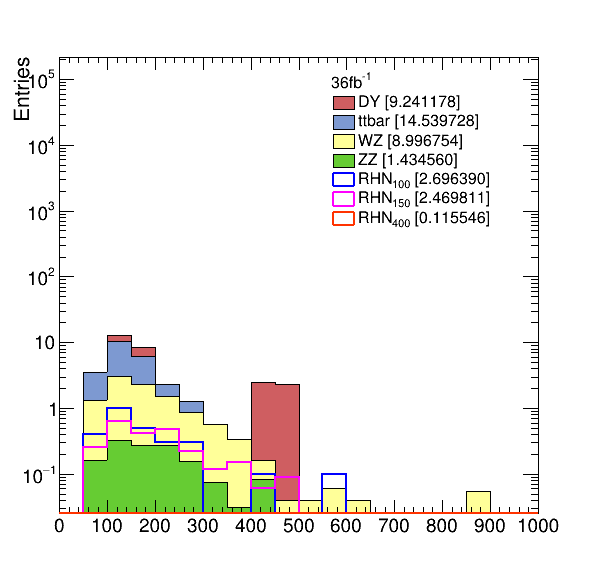
\includegraphics[trim=0 0 0 45,clip, width=0.45\textwidth]{images/2l1tc2lt.png} }}%
  \vspace{0.6cm}
  \tiny
  \setlength{\tabcolsep}{20pt}
  \renewcommand{\arraystretch}{1.6}
  \begin{tabular}{|c|c|}
    \hline
    Significance before cut & Significance after cut\\
    \hline
    \Gape[0.2cm]{\makecell{
        \sig{} $(100) = 0.2990$\\
        \sig{} $(150) = 0.3800$\\
        \sig{} $(400) = 0.0654$ }} & 
    \makecell{
      \sig{} $(100) = 0.4610$\\
      \sig{} $(150) = 0.4222$\\
      \sig{} $(400) = 0.0197$}\\
    \hline
  \end{tabular}
  \caption[\2l1t-OS Cut-2: \dphi{} (\ll, \ls) < 1]{\dphi{} (\ll, \ls) < 1 for \2l1t-OS \metpt $>50$ events.}
  \label{fig:2l1tc2}
  
\end{figure}

%cut 3
\begin{figure}[h!]
  \centering
  \makebox[0pt][c]{%
  \subfloat[{\scriptsize $m_{T}$ ($\tau$, \met) [\GeV]}]{{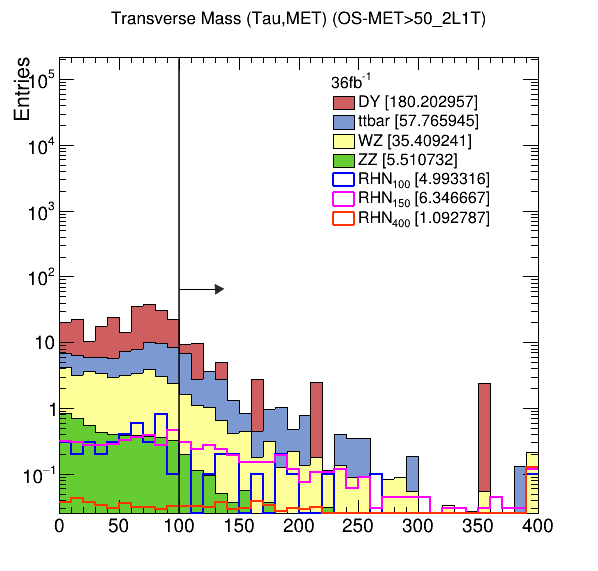
\includegraphics[trim=0 0 0 40,clip, width=0.35\textwidth]{images/2l1tc3.png} }}%
  \subfloat{{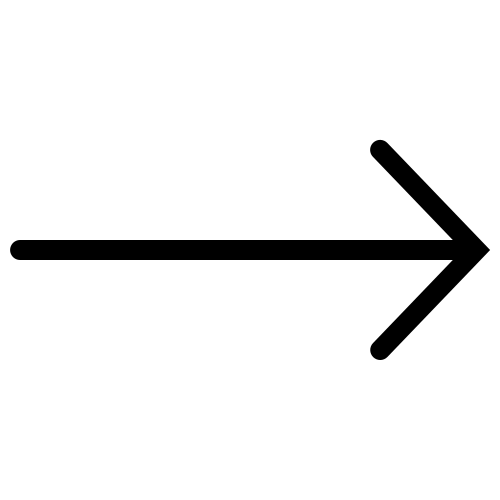
\includegraphics[trim=0 -1400 0 -1400,clip, height=5cm, width=0.05\textwidth]{images/right-arrow.png} }}%
  \subfloat[{\scriptsize \DeltaR{} (\ls, $\tau$)}]{{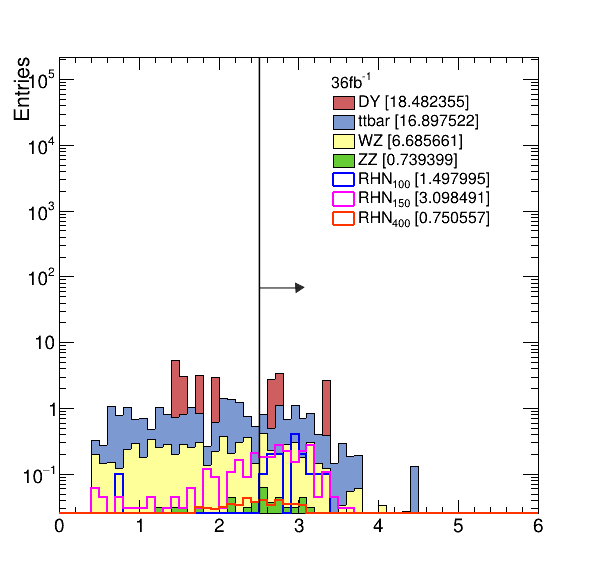
\includegraphics[trim=0 0 0 40,clip, width=0.35\textwidth]{images/2l1tc3-1.png} }}%
  \subfloat{{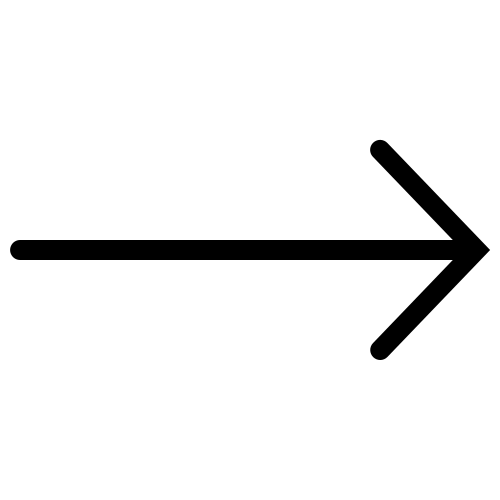
\includegraphics[trim=0 -1400 0 -1400,clip, height=5cm, width=0.05\textwidth]{images/right-arrow.png} }}%
  \subfloat[{\scriptsize \Lt{} [\GeV]}]{{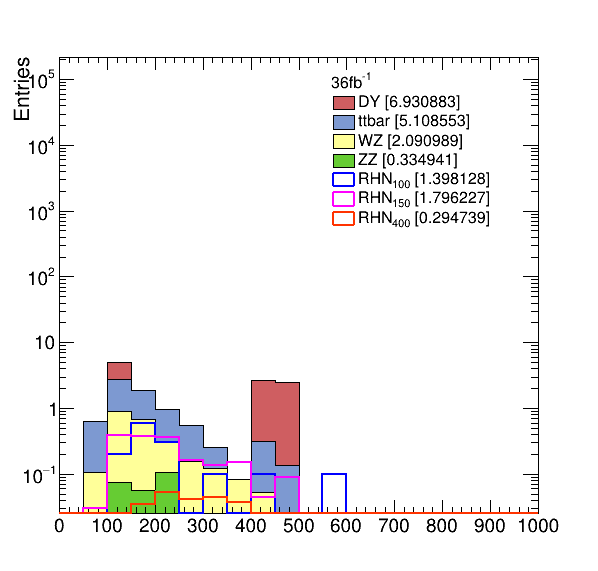
\includegraphics[trim=0 0 0 45,clip, width=0.35\textwidth]{images/2l1tc3lt.png} }}%
  }
  \makebox[\textwidth][c]{%
    \rule{0pt}{0.6cm}
    }
  \tiny
  \setlength{\tabcolsep}{20pt}
  \renewcommand{\arraystretch}{1.6}
  \begin{tabular}{|c|c|c|}
    \hline
    Significance before cuts & Significance after $m_{T}$ cut & Significance after \DeltaR{} cut\\
    \hline
    \Gape[0.2cm]{\makecell{
        \sig{} $(100) = 0.2990$\\
        \sig{} $(150) = 0.3800$\\
        \sig{} $(400) = 0.0654$ }} & 
    \makecell{
      \sig{} $(100) = 0.2289$\\
      \sig{} $(150) = 0.4736$\\
      \sig{} $(400) = 0.1147$} & 
    \makecell{
      \sig{} $(100) = 0.3676$\\
      \sig{} $(150) = 0.4723$\\
      \sig{} $(400) = 0.0774$}\\
    \hline
  \end{tabular}
  \caption[\2l1t-OS Cut-3: $m_{T}$ ($\tau$, \met) $> 100$ + \DeltaR{} (\ls, $\tau$) $>2.5$]{$m_{T}$ ($\tau$, \met) $> 100$ and \DeltaR{} (\ls, $\tau$) $>2.5$ for \2l1t-OS \metpt $>50$ events.}
  \label{fig:2l1tc3}
  \vspace{1cm}
\end{figure}

%cut 4
\begin{figure}[h!]
  \centering
  \makebox[0pt][c]{%
  \subfloat[{\scriptsize \pt{} of $\tau$ [\GeV]}]{{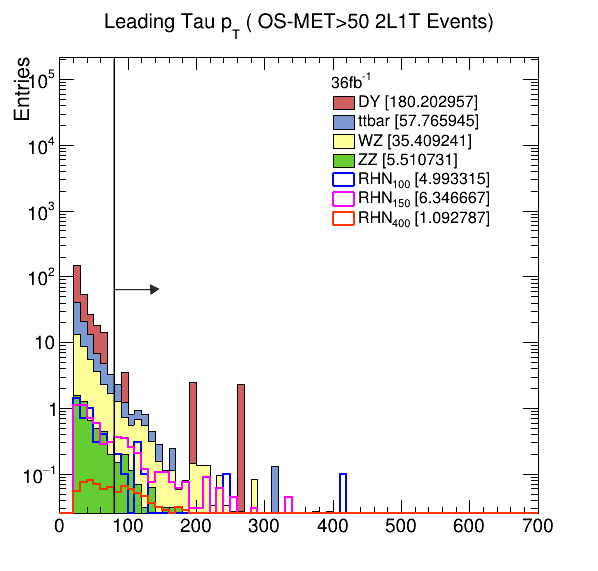
\includegraphics[trim=0 0 0 40,clip, width=0.35\textwidth]{images/2l1tc4.png} }}%
  \subfloat{{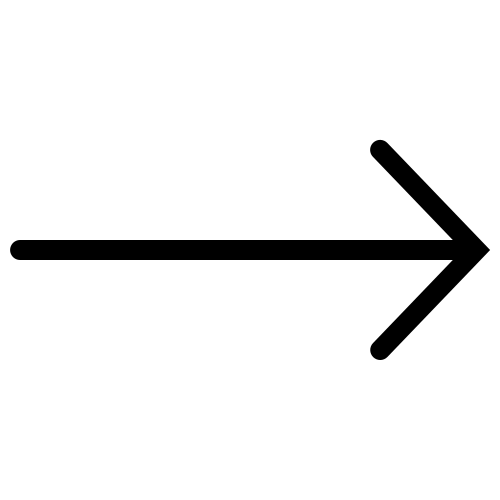
\includegraphics[trim=0 -1400 0 -1400,clip, height=5cm, width=0.05\textwidth]{images/right-arrow.png} }}%
  \subfloat[{\scriptsize \DeltaR{} (\ls, $\tau$)}]{{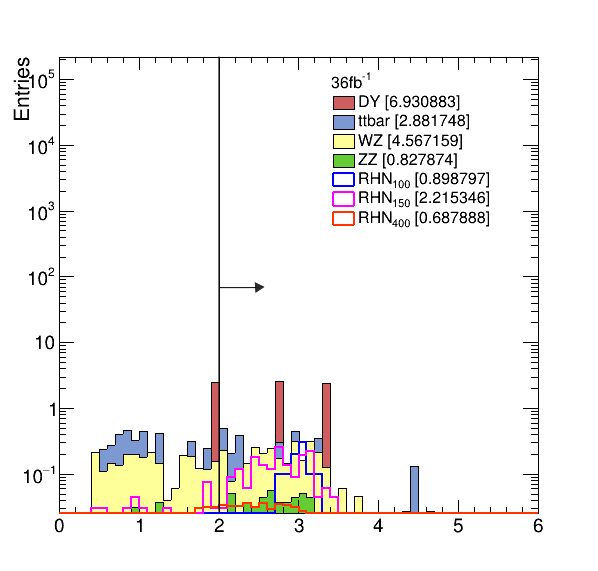
\includegraphics[trim=0 0 0 40,clip, width=0.35\textwidth]{images/2l1tc4-1.png} }}%
  \subfloat{{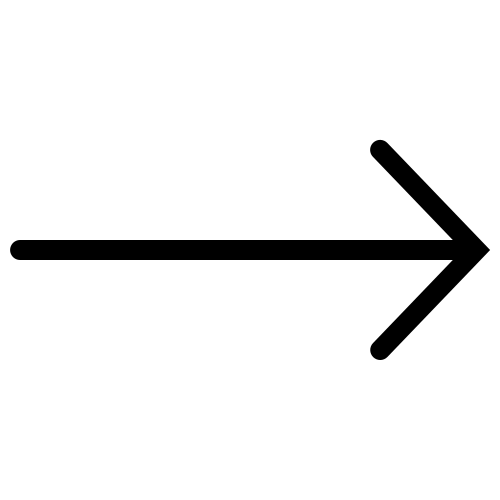
\includegraphics[trim=0 -1400 0 -1400,clip, height=5cm, width=0.05\textwidth]{images/right-arrow.png} }}%
  \subfloat[{\scriptsize \Lt{} [\GeV]}]{{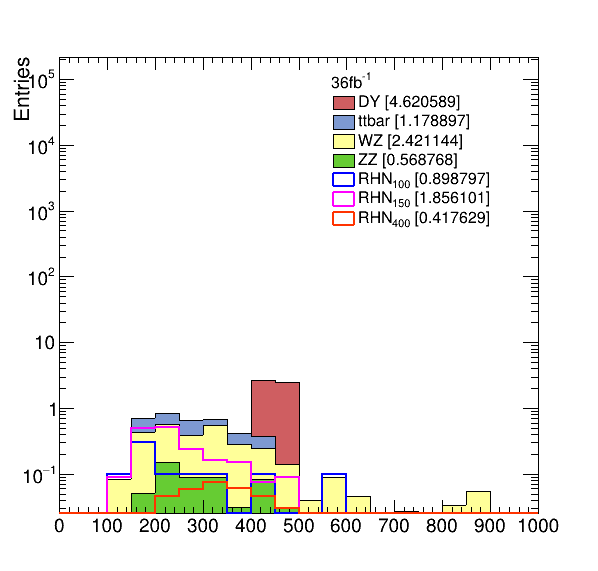
\includegraphics[trim=0 0 0 45,clip, width=0.35\textwidth]{images/2l1tc4lt.png} }}%
  }
  \makebox[\textwidth][c]{%
    \rule{0pt}{0.6cm}
    }
  \tiny
  \setlength{\tabcolsep}{20pt}
  \renewcommand{\arraystretch}{1.6}
  \begin{tabular}{|c|c|c|}
    \hline
    Significance before cuts & Significance after \pt{} cut & Significance after \DeltaR{} cut\\
    \hline
    \Gape[0.2cm]{\makecell{
        \sig{} $(100) = 0.2990$\\
        \sig{} $(150) = 0.3800$\\
        \sig{} $(400) = 0.0654$ }} & 
    \makecell{
      \sig{} $(100) = 0.2305$\\
      \sig{} $(150) = 0.5681$\\
      \sig{} $(400) = 0.1764$} & 
    \makecell{
      \sig{} $(100) = 0.3032$\\
      \sig{} $(150) = 0.6260$\\
      \sig{} $(400) = 0.1408$}\\
    \hline
  \end{tabular}
  \caption[\2l1t-OS Cut-4: \pt{} of $\tau$ $>80$ + \DeltaR{} (\ls, $\tau$) $>2$]{\pt{} of $\tau$ $>80$ and \DeltaR{} (\ls, $\tau$) $>2$ for \2l1t-OS \metpt $>50$ events.}
  \label{fig:2l1tc4}
  \vspace{4cm}
\end{figure}

%cut 5
\begin{figure}[h!]
  \centering
  \makebox[0pt][c]{%
  \subfloat[{\scriptsize \pt{} of $\tau$ [\GeV]}]{{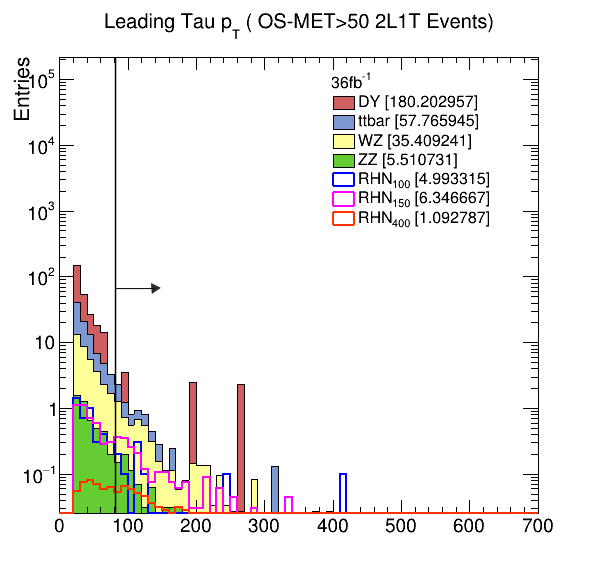
\includegraphics[trim=0 0 0 40,clip, width=0.35\textwidth]{images/2l1tc5.png} }}%
  \subfloat{{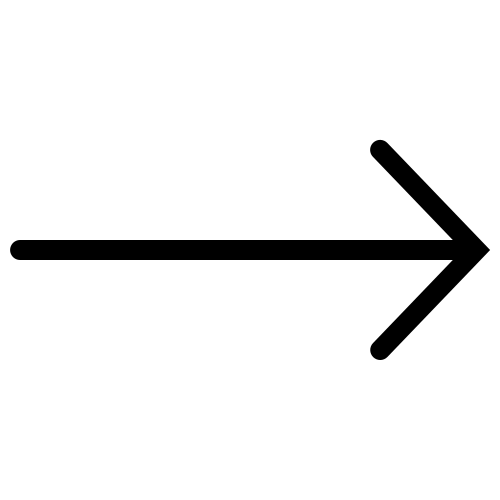
\includegraphics[trim=0 -1400 0 -1400,clip, height=5cm, width=0.05\textwidth]{images/right-arrow.png} }}%
  \subfloat[{\scriptsize \dphi{} (\ll, \ls)}]{{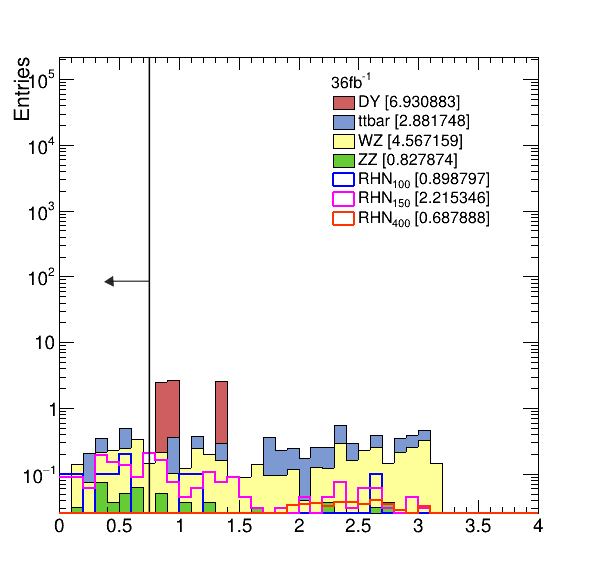
\includegraphics[trim=0 0 0 40,clip, width=0.35\textwidth]{images/2l1tc5-1.png} }}%
  \subfloat{{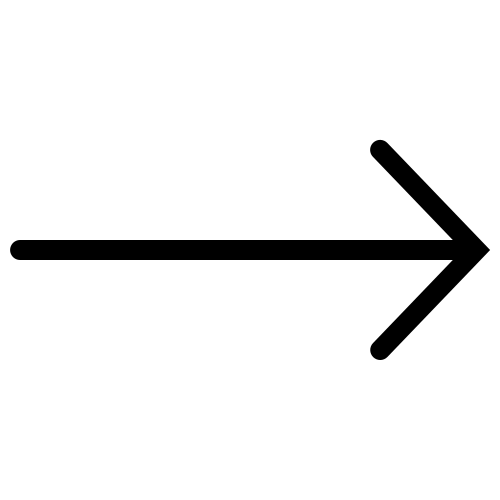
\includegraphics[trim=0 -1400 0 -1400,clip, height=5cm, width=0.05\textwidth]{images/right-arrow.png} }}%
  \subfloat[{\scriptsize \Lt{} [\GeV]}]{{\includegraphics[trim=0 0 0 45,clip, width=0.35\textwidth]{images/2l1tc5lt.png} }}%
  }
  \makebox[\textwidth][c]{%
    \rule{0pt}{0.6cm}
    }
  \tiny
  \setlength{\tabcolsep}{20pt}
  \renewcommand{\arraystretch}{1.6}
  \begin{tabular}{|c|c|c|}
    \hline
    Significance before cuts & Significance after \pt{} cut & Significance after \dphi{} cut\\
    \hline
    \Gape[0.2cm]{\makecell{
        \sig{} $(100) = 0.2990$\\
        \sig{} $(150) = 0.3800$\\
        \sig{} $(400) = 0.0654$ }} & 
    \makecell{
      \sig{} $(100) = 0.2305$\\
      \sig{} $(150) = 0.5681$\\
      \sig{} $(400) = 0.1764$} & 
    \makecell{
      \sig{} $(100) = 0.4426$\\
      \sig{} $(150) = 0.6855$\\
      \sig{} $(400) = 0.0452$}\\
    \hline
  \end{tabular}
  \caption[\2l1t-OS Cut-5: \pt{} of $\tau$ $>80$ + \dphi{} (\ll, \ls) $< 0.75$]{\pt{} of $\tau$ $>80$ and \dphi{} (\ll, \ls) $< 0.75$ for \2l1t-OS \metpt $>50$ events.}
  \label{fig:2l1tc5}
\end{figure}
\vspace{1.5cm}

As expected, the \DeltaR{} variables are important and selecting regions based on them can give us good signinificance for all the mass points. We therefore plot 2-D histograms with these variables on one axis. Different regions on the 2-D plane can then be selected as signal regions. These plots are shown in Figures~\ref{fig:2l1t2d1} to \ref{fig:2l1t2d3}.

%2d1
\captionsetup[subfigure]{labelformat=empty}
\begin{figure}[h!]
  \centering
  \makebox[0pt][c]{
    \subfloat[{\scriptsize $m_{T} (\tau, \met)$ v/s \DeltaR{} (\ll, \ls) ($100\GeV$)}]{{\includegraphics[trim=0 0 0 25,clip, width=0.4\textwidth]{images/2l1t-2d/1-100.png} }}%
    \enskip
    \subfloat[{\scriptsize $m_{T} (\tau, \met)$ v/s \DeltaR{} (\ll, \ls) ($150\GeV$)}]{{\includegraphics[trim=0 0 0 25,clip, width=0.4\textwidth]{images/2l1t-2d/1-150.png} }}%
    \enskip
    \subfloat[{\scriptsize $m_{T} (\tau, \met)$ v/s \DeltaR{} (\ll, \ls) ($400\GeV$)}]{{\includegraphics[trim=0 0 0 25,clip, width=0.4\textwidth]{images/2l1t-2d/1-400.png} }}%
  }
  \makebox[\textwidth][c]{
    \rule{0pt}{0.2cm}
  }
  \makebox[0pt][c]{
    \subfloat[{\scriptsize DY}]{{\includegraphics[trim=0 0 0 25,clip,width=0.27\textwidth]{images/2l1t-2d/1-dy.png} }}%
    \enskip
    \subfloat[{\scriptsize \ttbar}]{{\includegraphics[trim=0 0 0 25,clip,width=0.27\textwidth]{images/2l1t-2d/1-ttbar.png}}}%
    \enskip
    \subfloat[{\scriptsize \WZ}]{{\includegraphics[trim=0 0 0 25,clip, width=0.27\textwidth]{images/2l1t-2d/1-wz.png} }}%
    \subfloat[{\scriptsize \ZZ}]{{\includegraphics[trim=0 0 0 25,clip, width=0.27\textwidth]{images/2l1t-2d/1-zz.png} }}%
  }
  \makebox[\textwidth][c]{
    \rule{0pt}{0.2cm}
  }
  \makebox[\textwidth][c]{
    \tiny
    \setlength{\tabcolsep}{20pt}
    \renewcommand{\arraystretch}{1.6}
    \begin{tabular}{|c|c|}
      \hline
      Significance before cuts & Significance after cuts\\
      \hline
      \Gape[0.2cm]{\makecell{
          \sig{} $(100) = 0.2990$\\
          \sig{} $(150) = 0.3800$\\
          \sig{} $(400) = 0.0654$ }} & 
      \makecell{
        \sig{} $(100) = 0.443$ [bin $(1,1)$]\\
        \sig{} $(150) = 0.376$ [bin $(1,2)$]\\
        \sig{} $(400) = 0.110$ [bin $(2,2)$]}\\
    \hline
    \end{tabular}
  }
  \caption[(\2l1t-OS 2-D histogram) $m_{T} (\tau, \met)$ v/s \DeltaR{} (\ll, \ls)]{[\2l1t-OS 2-D histogram] $m_{T} (\tau, \met)$ v/s \DeltaR{} (\ll, \ls) (all $m_{T}$ axes are in \GeV{} units). The bins (x,y) with the best significance for each mass point have been mentioned in parentheses.}
  \label{fig:2l1t2d1}
  \vspace{0.4cm}
\end{figure}

%2d2
\captionsetup[subfigure]{labelformat=empty}
\begin{figure}[h!]
  \centering
  \makebox[0pt][c]{
    \subfloat[{\scriptsize $\tau$ \pt{} v/s \DeltaR{} (\ll, \ls) ($100\GeV$)}]{{\includegraphics[trim=0 0 0 25,clip, width=0.4\textwidth]{images/2l1t-2d/2-100.png} }}%
    \enskip
    \subfloat[{\scriptsize $\tau$ \pt{} v/s \DeltaR{} (\ll, \ls) ($150\GeV$)}]{{\includegraphics[trim=0 0 0 25,clip, width=0.4\textwidth]{images/2l1t-2d/2-150.png} }}%
    \enskip
    \subfloat[{\scriptsize $\tau$ \pt{} v/s \DeltaR{} (\ll, \ls) ($400\GeV$)}]{{\includegraphics[trim=0 0 0 25,clip, width=0.4\textwidth]{images/2l1t-2d/2-400.png} }}%
  }
  \makebox[\textwidth][c]{
    \rule{0pt}{0.2cm}
  }
  \makebox[0pt][c]{
    \subfloat[{\scriptsize DY}]{{\includegraphics[trim=0 0 0 25,clip,width=0.27\textwidth]{images/2l1t-2d/2-dy.png} }}%
    \enskip
    \subfloat[{\scriptsize \ttbar}]{{\includegraphics[trim=0 0 0 25,clip,width=0.27\textwidth]{images/2l1t-2d/2-ttbar.png}}}%
    \enskip
    \subfloat[{\scriptsize \WZ}]{{\includegraphics[trim=0 0 0 25,clip, width=0.27\textwidth]{images/2l1t-2d/2-wz.png} }}%
    \subfloat[{\scriptsize \ZZ}]{{\includegraphics[trim=0 0 0 25,clip, width=0.27\textwidth]{images/2l1t-2d/2-zz.png} }}%
  }
  \makebox[\textwidth][c]{
    \rule{0pt}{0.2cm}
  }
  \makebox[\textwidth][c]{
    \tiny
    \setlength{\tabcolsep}{20pt}
    \renewcommand{\arraystretch}{1.6}
    \begin{tabular}{|c|c|}
      \hline
      Significance before cuts & Significance after cuts\\
      \hline
      \Gape[0.2cm]{\makecell{
          \sig{} $(100) = 0.2990$\\
          \sig{} $(150) = 0.3800$\\
          \sig{} $(400) = 0.0654$ }} & 
      \makecell{
        \sig{} $(100) = 0.416$ [bin $(1,2)$]\\
        \sig{} $(150) = 0.425$ [bin $(1,2)$]\\
        \sig{} $(400) = 0.117$ [bin $(2,2)$]}\\
    \hline
    \end{tabular}
  }
  \caption[(\2l1t-OS 2-D histogram) $\tau$ \pt{} v/s \DeltaR{} (\ll, \ls)]{[\2l1t-OS 2-D histogram] $\tau$ \pt{} v/s \DeltaR{} (\ll, \ls) (all \pt{} axes are in \GeV{} units). The bins (x,y) with the best significance for each mass point have been mentioned in parentheses.}
  \label{fig:2l1t2d2}
\end{figure}

%2d3
\captionsetup[subfigure]{labelformat=empty}
\begin{figure}[h!]
  \centering
  \makebox[0pt][c]{
    \subfloat[{\scriptsize $m_{T} (\tau, \met)$ v/s \DeltaR{} (\ls, $\tau$) ($100\GeV$)}]{{\includegraphics[trim=0 0 0 25,clip, width=0.4\textwidth]{images/2l1t-2d/3-100.png} }}%
    \enskip
    \subfloat[{\scriptsize $m_{T} (\tau, \met)$ v/s \DeltaR{} (\ls, $\tau$) ($150\GeV$)}]{{\includegraphics[trim=0 0 0 25,clip, width=0.4\textwidth]{images/2l1t-2d/3-150.png} }}%
    \enskip
    \subfloat[{\scriptsize $m_{T} (\tau, \met)$ v/s \DeltaR{} (\ls, $\tau$) ($400\GeV$)}]{{\includegraphics[trim=0 0 0 25,clip, width=0.4\textwidth]{images/2l1t-2d/3-400.png} }}%
  }
  \makebox[\textwidth][c]{
    \rule{0pt}{0.2cm}
  }
  \makebox[0pt][c]{
    \subfloat[{\scriptsize DY}]{{\includegraphics[trim=0 0 0 25,clip,width=0.27\textwidth]{images/2l1t-2d/3-dy.png} }}%
    \enskip
    \subfloat[{\scriptsize \ttbar}]{{\includegraphics[trim=0 0 0 25,clip,width=0.27\textwidth]{images/2l1t-2d/3-ttbar.png}}}%
    \enskip
    \subfloat[{\scriptsize \WZ}]{{\includegraphics[trim=0 0 0 25,clip, width=0.27\textwidth]{images/2l1t-2d/3-wz.png} }}%
    \subfloat[{\scriptsize \ZZ}]{{\includegraphics[trim=0 0 0 25,clip, width=0.27\textwidth]{images/2l1t-2d/3-zz.png} }}%
  }
  \makebox[\textwidth][c]{
    \rule{0pt}{0.2cm}
  }
  \makebox[\textwidth][c]{
    \tiny
    \setlength{\tabcolsep}{20pt}
    \renewcommand{\arraystretch}{1.6}
    \begin{tabular}{|c|c|}
      \hline
      Significance before cuts & Significance after cuts\\
      \hline
      \Gape[0.2cm]{\makecell{
          \sig{} $(100) = 0.2990$\\
          \sig{} $(150) = 0.3800$\\
          \sig{} $(400) = 0.0654$ }} & 
      \makecell{
        \sig{} $(100) = 0.342$ [bin $(2,2)$]\\
        \sig{} $(150) = 0.450$ [bin $(2,2)$]\\
        \sig{} $(400) = 0.075$ [bin $(1,2)$]}\\
    \hline
    \end{tabular}
  }
  \caption[(\2l1t-OS 2-D histogram) $m_{T} (\tau, \met)$ v/s \DeltaR{} (\ls, $\tau$)]{[\2l1t-OS 2-D histogram] $m_{T} (\tau, \met)$ v/s \DeltaR{} (\ls, $\tau$) (all $m_{T}$ axes are in \GeV{} units). The bins (x,y) with the best significance for each mass point have been mentioned in parentheses.}
  \label{fig:2l1t2d3}
  \vspace{0.4cm}
  \makebox[0pt][c]{
  }
\end{figure}

\subsubsection{{\Large{\boldmath$2\ell1\tau$} - SS}}
\label{sec:2l1tSS}

Following a strategy similar to that of the \2l1t-OS channel, we look at the basic \pt, \DeltaR, $m_{T}$ and \Lt{} plots [Figure~\ref{fig:2l1tSSplots}] and then apply the appropriate selections. We try a number of cuts on newly introduced variables specific to this channel (like \DeltaR{} between the same-sign lepton pair). We also make cuts based on the presence of an OS lepton pair. Unfortunately, none of the selections give a significance better than the initial one. The optimal signal region seems to be the region with events that have an OS pair. A summary of all the selections is given in Table~\ref{tab:2l1t}.

%SS plots
\begin{figure}[h!]
  \centering
  \makebox[0pt][c]{%
  \subfloat[{\scriptsize \pt{} of leading light lepton \ll [\GeV]}]{{\includegraphics[trim=0 0 0 45,clip, width=0.35\textwidth]{images/ss/llpt.png}}}
  \enskip
  \subfloat[{\scriptsize \pt{} of sub-leading light lepton \ls [\GeV]}]{{\includegraphics[trim=0 0 0 45,clip, width=0.35\textwidth]{images/ss/slpt.png} }}%
  \enskip
  \subfloat[{\scriptsize \pt{} of $\tau$ [\GeV]}]{{\includegraphics[trim=0 0 0 45,clip, width=0.35\textwidth]{images/ss/tpt.png} }}%
  }
  \makebox[\textwidth][c]{%
    \rule{0pt}{0.4cm}
    }
  \makebox[0pt][c]{%
  \subfloat[{\scriptsize \DeltaR{} (\ll,\ls)}]{{\includegraphics[trim=0 0 0 45,clip, width=0.35\textwidth]{images/ss/dR0.png} }}%
  \enskip
  \subfloat[{\scriptsize \DeltaR{} (\ll,$\tau$)}]{{\includegraphics[trim=0 0 0 45,clip, width=0.35\textwidth]{images/ss/dR1.png} }}%
  \enskip
  \subfloat[{\scriptsize \DeltaR{} (\ls,$\tau$)}]{{\includegraphics[trim=0 0 0 45,clip, width=0.35\textwidth]{images/ss/dR2.png} }}%
  }
  \makebox[\textwidth][c]{%
    \rule{0pt}{0.4cm}
    }
  \makebox[0pt][c]{%
    \subfloat[{\scriptsize \Lt{} [\GeV]}]{{\includegraphics[trim=0 0 0 45,clip, width=0.35\textwidth]{images/ss/Lt.png}}}
    \qquad
    \subfloat[{\scriptsize $m_{T}$ ($\tau$, \met) [\GeV]}]{{\includegraphics[trim=0 0 0 45,clip, width=0.35\textwidth]{images/ss/mt0.png} }}%
  }
  \caption{Some basic distributions for the \2l1t-SS region.}
  \label{fig:2l1tSSplots}
\end{figure}

%cut 1
\begin{figure}[h!]
  \centering
  \subfloat[{\scriptsize \DeltaR{} (\ll,\ls)}]{{\includegraphics[trim=0 0 0 40,clip, width=0.45\textwidth]{images/ss/2l1tc1.png} }}%
  \subfloat{{\includegraphics[trim=0 -1400 0 -1400,clip, height=7cm, width=0.1\textwidth]{images/right-arrow.png} }}%
  \subfloat[{\scriptsize \Lt{} [\GeV]}]{{\includegraphics[trim=0 0 0 45,clip, width=0.45\textwidth]{images/ss/2l1tc1lt.png} }}%
  \vspace{0.6cm}
  \tiny
  \setlength{\tabcolsep}{20pt}
  \renewcommand{\arraystretch}{1.6}
  \begin{tabular}{|c|c|}
    \hline
    Significance before cut & Significance after cut\\
    \hline
    \Gape[0.2cm]{\makecell{
        \sig{} $(100) = 0.3339$\\
        \sig{} $(150) = 0.5645$\\
        \sig{} $(400) = 0.0618$ }} & 
    \makecell{
      \sig{} $(100) = 0.3021$\\
      \sig{} $(150) = 0.5263$\\
      \sig{} $(400) = 0.0512$}\\
    \hline
  \end{tabular}
  \caption[\2l1t-SS Cut-1: \DeltaR{} (\ll,\ls) $> 2.4$]{\DeltaR{} (\ll,\ls) $> 2.4$ for \2l1t-SS channel.}
  \label{fig:ss2l1tc1}
\end{figure}

%cut 2
\begin{figure}[h!]
  \centering
  \subfloat[{\scriptsize \dphi{} (\ll,\ls)}]{{\includegraphics[trim=0 0 0 40,clip, width=0.45\textwidth]{images/ss/2l1tc2.png} }}%
  \subfloat{{\includegraphics[trim=0 -1400 0 -1400,clip, height=7cm, width=0.1\textwidth]{images/right-arrow.png} }}%
  \subfloat[{\scriptsize \Lt{} [\GeV]}]{{\includegraphics[trim=0 0 0 45,clip, width=0.45\textwidth]{images/ss/2l1tc2lt.png} }}%
  \vspace{0.6cm}
  \tiny
  \setlength{\tabcolsep}{20pt}
  \renewcommand{\arraystretch}{1.6}
  \begin{tabular}{|c|c|}
    \hline
    Significance before cut & Significance after cut\\
    \hline
    \Gape[0.2cm]{\makecell{
        \sig{} $(100) = 0.3339$\\
        \sig{} $(150) = 0.5645$\\
        \sig{} $(400) = 0.0618$ }} & 
    \makecell{
      \sig{} $(100) = 0.3441$\\
      \sig{} $(150) = 0.5127$\\
      \sig{} $(400) = 0.0468$}\\
    \hline
  \end{tabular}
  \caption[\2l1t-SS Cut-2: \dphi{} (\ll,\ls) $> 2.3$]{\dphi{} (\ll,\ls) $> 2.3$ for \2l1t-SS channel.}
  \label{fig:ss2l1tc2}
\end{figure}

%cut 3
\begin{figure}[h!]
  \centering
  \subfloat[{\scriptsize \DeltaR{} (\ls, $\tau$)}]{{\includegraphics[trim=0 0 0 40,clip, width=0.45\textwidth]{images/ss/2l1tc3.png} }}%
  \subfloat{{\includegraphics[trim=0 -1400 0 -1400,clip, height=7cm, width=0.1\textwidth]{images/right-arrow.png} }}%
  \subfloat[{\scriptsize \Lt{} [\GeV]}]{{\includegraphics[trim=0 0 0 45,clip, width=0.45\textwidth]{images/ss/2l1tc3lt.png} }}%
  \vspace{0.6cm}
  \tiny
  \setlength{\tabcolsep}{20pt}
  \renewcommand{\arraystretch}{1.6}
  \begin{tabular}{|c|c|}
    \hline
    Significance before cut & Significance after cut\\
    \hline
    \Gape[0.2cm]{\makecell{
        \sig{} $(100) = 0.3339$\\
        \sig{} $(150) = 0.5645$\\
        \sig{} $(400) = 0.0618$ }} & 
    \makecell{
      \sig{} $(100) = 0.2388$\\
      \sig{} $(150) = 0.4074$\\
      \sig{} $(400) = 0.0329$}\\
    \hline
  \end{tabular}
  \caption[\2l1t-SS Cut-3: \DeltaR{} (\ls,$\tau$) $< 2$]{\DeltaR{} (\ls,$\tau$) $< 2$ for \2l1t-SS channel.}
  \label{fig:ss2l1tc3}
\end{figure}

%2d1
\captionsetup[subfigure]{labelformat=empty}
\begin{figure}[h!]
  \centering
  \makebox[0pt][c]{
    \subfloat[{\scriptsize \Lt{} v/s \DeltaR{} (\ll, \ls) ($100\GeV$)}]{{\includegraphics[trim=0 0 0 25,clip, width=0.4\textwidth]{images/ss/1-100.png} }}%
    \enskip
    \subfloat[{\scriptsize \Lt{} v/s \DeltaR{} (\ll, \ls) ($150\GeV$)}]{{\includegraphics[trim=0 0 0 25,clip, width=0.4\textwidth]{images/ss/1-150.png} }}%
    \enskip
    \subfloat[{\scriptsize \Lt{} v/s \DeltaR{} (\ll, \ls) ($400\GeV$)}]{{\includegraphics[trim=0 0 0 25,clip, width=0.4\textwidth]{images/ss/1-400.png} }}%
  }
  \makebox[\textwidth][c]{
    \rule{0pt}{0.2cm}
  }
  \makebox[0pt][c]{
    \subfloat[{\scriptsize DY}]{{\includegraphics[trim=0 0 0 25,clip,width=0.27\textwidth]{images/ss/1-dy.png} }}%
    \enskip
    \subfloat[{\scriptsize \ttbar}]{{\includegraphics[trim=0 0 0 25,clip,width=0.27\textwidth]{images/ss/1-ttbar.png}}}%
    \enskip
    \subfloat[{\scriptsize \WZ}]{{\includegraphics[trim=0 0 0 25,clip, width=0.27\textwidth]{images/ss/1-wz.png} }}%
    \subfloat[{\scriptsize \ZZ}]{{\includegraphics[trim=0 0 0 25,clip, width=0.27\textwidth]{images/ss/1-zz.png} }}%
  }
  \makebox[\textwidth][c]{
    \rule{0pt}{0.2cm}
  }
  \makebox[\textwidth][c]{
    \tiny
    \setlength{\tabcolsep}{20pt}
    \renewcommand{\arraystretch}{1.6}
    \begin{tabular}{|c|c|}
      \hline
      Significance before cuts & Significance after cuts\\
      \hline
      \Gape[0.2cm]{\makecell{
          \sig{} $(100) = 0.3339$\\
          \sig{} $(150) = 0.5645$\\
          \sig{} $(400) = 0.0618$ }} & 
      \makecell{
        \sig{} $(100) = 0.317$ [bin $(2,2)$]\\
        \sig{} $(150) = 0.501$ [bin $(2,2)$]\\
        \sig{} $(400) = 0.093$ [bin $(2,2)$]}\\
    \hline
    \end{tabular}
  }
  \caption[(\2l1t-SS 2-D histogram) \Lt{} v/s \DeltaR{} (\ll, \ls)]{[\2l1t-SS 2-D histogram] \Lt{} v/s \DeltaR{} (\ll, \ls) (all \Lt{} axes are in \GeV{} units). The bins (x,y) with the best significance for each mass point have been mentioned in parentheses.}
  \label{fig:ss2l1t2d}
  \vspace{0.4cm}
\end{figure}

%summary table
\begin{table}[h]
  \centering
  \large
  \setlength{\tabcolsep}{20pt}
  \renewcommand{\arraystretch}{2}
  \resizebox{\textwidth}{!}{%
    \begin{tabular}{r|l|r|r|r}
    \hline \hline
    &Selection & \multicolumn{1}{r|}{\sig{} $(100)$} & \multicolumn{1}{r|}{\sig{} $(150)$} & \multicolumn{1}{r}{\sig{} $(400)$}\\
    \hline
\multirow{3}{*}{\begin{sideways}\2l1t-OS \end{sideways}} & $\pt^{miss} >50$ + \DeltaR{} (\ll, \ls) $<1.5$  & $0.4811$ & $0.4675$ & $0.0176$\\
& $\pt^{miss} >50$ + \pt($\tau$) $>80$ + \dphi{} (\ll, \ls) $<0.75$ & \colorbox{yellow}{\boldmath $0.4426$} & \colorbox{yellow}{\boldmath $0.6855$} & \colorbox{yellow}{\boldmath $0.0452$}\\
& $\pt^{miss} >50$ [2-D histogram]  \pt($\tau$) v/s \DeltaR{} (\ll, \ls)  & $0.416$ & $0.425$ & $0.117$\\
\hline
\multirow{3}{*}{\begin{sideways}\2l1t-SS \end{sideways}} & Events with an OS pair & \colorbox{yellow}{\boldmath $0.3657$} & \colorbox{yellow}{\boldmath $0.6417$} & \colorbox{yellow}{\boldmath $0.0693$}\\
& \dphi{} (\ll, \ls) $>2.3$ & $0.3441$ & $0.5127$ & $0.0468$\\
& [2-D histogram] \Lt{} v/s \DeltaR{} (\ll, \ls)  & $0.317$ & $0.501$ & $0.093$\\
\hline \hline
    \end{tabular}%
    }
  \caption{Summary table for the \2l1t{} channel.}
  \label{tab:2l1t}
\end{table}

\subsection{\Large{\boldmath$3\ell$}}
\label{sec:3l}

The \3l channel is similar to the \2l1t{} channel in terms of event topology (we have a light lepton fake instead of a $\tau$ fake). \3l{} has fewer events than the \2l1t channel (after applying vetoes). In addition to that, there is a lot of background (majorly DY and \WZ). So, for this part of the analysis, we start by dividing the channel into 7 categories based on the sign (S) and flavour (F) of each lepton and where it lies with respect to the on-\Zboson{} range:

\begin{enumerate}
\item OSSF Below-\Zboson
\item OSSF Above-\Zboson
\item SSSF Below-\Zboson
\item SSSF Above-\Zboson
\item OSOF Below-\Zboson
\item OSOF Above-\Zboson
\item All same-sign leptons
\end{enumerate}

Here, the below-\Zboson{} and above-\Zboson{} is defined as $<76\GeV$ and $>106\GeV$ respectively. After analyzing a couple of basic plots from each of these categories, we discard the ones which have very less signal (like SSSF and all same-sign categories). Finally, we are left with two categories: \emph{(1)} OSSF Below-\Zboson{} and \emph{(2)} OSOF Below-\Zboson.

\subsubsection{OSSF Below-{\boldmath \Zboson}}
\label{sec:ossf}

All the events that have at least one opposite-sign same-flavour (OSSF) pair belong to this category. In a lot of cases, we have an ambiguity since two such pairs can be formed (this is also true when we apply vetoes). To resolve this ambiguity, we pick the pair that is closer to the \Zboson{} mass, \ie{} we check $|M_{\ell^{+}\ell^{-}} - 91|$ and choose the OSSF pair for which this quantity is minimum. The third lepton is named the odd lepton. Some basic distributions are shown in Figure~\ref{fig:3lOSSFplots} and a summary of the best set of cuts is given in Table~\ref{tab:3l}.

%OSSF plots
\begin{figure}[h!]
  \centering
  \makebox[0pt][c]{%
  \subfloat[{\scriptsize \pt{} of leading light lepton \ll [\GeV]}]{{\includegraphics[trim=0 0 0 45,clip, width=0.35\textwidth]{images/3lossf/llpt.png}}}
  \enskip
  \subfloat[{\scriptsize \pt{} of sub-leading light lepton \ls [\GeV]}]{{\includegraphics[trim=0 0 0 45,clip, width=0.35\textwidth]{images/3lossf/slpt.png} }}%
  \enskip
  \subfloat[{\scriptsize \pt{} of sub-sub-leading lepton \lss [\GeV]}]{{\includegraphics[trim=0 0 0 45,clip, width=0.35\textwidth]{images/3lossf/sslpt.png} }}%
  }
  \makebox[\textwidth][c]{%
    \rule{0pt}{0.4cm}
    }
  \makebox[0pt][c]{%
  \subfloat[{\scriptsize \pt{} of odd lepton \lodd [\GeV]}]{{\includegraphics[trim=0 0 0 45,clip, width=0.35\textwidth]{images/3lossf/oddpt.png} }}%
  \enskip
  \subfloat[{\scriptsize \DeltaR{} (\ll,\ls)}]{{\includegraphics[trim=0 0 0 45,clip, width=0.35\textwidth]{images/3lossf/dR0.png} }}%
  \enskip
  \subfloat[{\scriptsize \DeltaR{} (OSSF pair)}]{{\includegraphics[trim=0 0 0 45,clip, width=0.35\textwidth]{images/3lossf/dRossf.png} }}%
  }
  \makebox[\textwidth][c]{%
    \rule{0pt}{0.4cm}
    }
  \makebox[0pt][c]{%
    \subfloat[{\scriptsize \Lt{} [\GeV]}]{{\includegraphics[trim=0 0 0 45,clip, width=0.45\textwidth]{images/3lossf/Lt.png}}}
    \qquad
    \subfloat[{\scriptsize \ptmiss{} [\GeV]}]{{\includegraphics[trim=0 0 0 45,clip, width=0.45\textwidth]{images/3lossf/metpt.png} }}%
  }
  \caption[Some basic distributions for the \3l-OSSF below-\Zboson{} channel]{Some basic distributions for the \3l-OSSF below-\Zboson{} channel. From the \pt{} plots, we observe that the odd lepton is often the leading lepton, \ie{} the OSSF pair is often of the lower \pt{} leptons. }
  \label{fig:3lOSSFplots}
  \vspace{1cm}
\end{figure}

%cut 1
\begin{figure}[h!]
  \centering
  \makebox[0pt][c]{%
  \subfloat[{\scriptsize \DeltaR{} (OSSF pair)}]{{\includegraphics[trim=0 0 0 40,clip, width=0.35\textwidth]{images/3lossf/3lc1-1.png} }}%
  \subfloat{{\includegraphics[trim=0 -2700 0 -2700,clip, height=5cm, width=0.05\textwidth]{images/plus.png} }}%
  \subfloat[{\scriptsize \ptmiss{} [\GeV]}]{{\includegraphics[trim=0 0 0 40,clip, width=0.35\textwidth]{images/3lossf/3lc1-2.png} }}%
  \subfloat{{\includegraphics[trim=0 -1400 0 -1400,clip, height=5cm, width=0.05\textwidth]{images/right-arrow.png} }}%
  \subfloat[{\scriptsize \Lt{} [\GeV]}]{{\includegraphics[trim=0 0 0 45,clip, width=0.35\textwidth]{images/3lossf/3lc1lt.png} }}%
  }
  \makebox[\textwidth][c]{%
    \rule{0pt}{0.6cm}
    }
  \tiny
  \setlength{\tabcolsep}{20pt}
  \renewcommand{\arraystretch}{1.6}
  \begin{tabular}{|c|c|}
    \hline
    Significance before cuts & Significance after cuts\\
    \hline
    \Gape[0.2cm]{\makecell{
        \sig{} $(100) = 0.1192$\\
        \sig{} $(150) = 0.0940$\\
        \sig{} $(400) = 0.0023$ }} & 
    \makecell{
      \sig{} $(100) = 0.1446$\\
      \sig{} $(150) = 0.1056$\\
      \sig{} $(400) = 0.0039$}\\
    \hline
  \end{tabular}
  \caption[\3l-OSSF Cut-1: \DeltaR{} (OSSF pair) $<2$ and \ptmiss{} $>50$]{\DeltaR{} (OSSF pair) $<2$ and \ptmiss{} $>50$ for \3l-OSSF below-\Zboson{} events.}
  \label{fig:3lc1}
  \vspace{1cm}
\end{figure}

%cut 3
\begin{figure}[h!]
  \centering
  \makebox[0pt][c]{%
  \subfloat[{\scriptsize $m_{T}$ (\ll, \met) [\GeV]}]{{\includegraphics[trim=0 0 0 40,clip, width=0.35\textwidth]{images/3lossf/3lc3-1.png} }}%
  \subfloat{{\includegraphics[trim=0 -2700 0 -2700,clip, height=5cm, width=0.05\textwidth]{images/plus.png} }}%
  \subfloat[{\scriptsize \dphi{} (\lodd, $\ell_{OSSF_{1}}$)}]{{\includegraphics[trim=0 0 0 40,clip, width=0.35\textwidth]{images/3lossf/3lc3-2.png} }}%
  \subfloat{{\includegraphics[trim=0 -1400 0 -1400,clip, height=5cm, width=0.05\textwidth]{images/right-arrow.png} }}%
  \subfloat[{\scriptsize \Lt{} [\GeV]}]{{\includegraphics[trim=0 0 0 45,clip, width=0.35\textwidth]{images/3lossf/3lc3lt.png} }}%
  }
  \makebox[\textwidth][c]{%
    \rule{0pt}{0.6cm}
    }
  \tiny
  \setlength{\tabcolsep}{20pt}
  \renewcommand{\arraystretch}{1.6}
  \begin{tabular}{|c|c|}
    \hline
    Significance before cuts & Significance after cuts\\
    \hline
    \Gape[0.2cm]{\makecell{
        \sig{} $(100) = 0.1192$\\
        \sig{} $(150) = 0.0940$\\
        \sig{} $(400) = 0.0023$ }} & 
    \makecell{
      \sig{} $(100) = 0.1828$\\
      \sig{} $(150) = 0.1497$\\
      \sig{} $(400) = 0.0055$}\\
    \hline
  \end{tabular}
  \caption[\3l-OSSF Cut-2: $m_{T}$ (\ll, \met) $>80$ and \dphi{} (\lodd, $\ell_{OSSF_{1}}$) $>2.5$]{ $m_{T}$ (\ll, \met) $>80$ and \dphi{} (\lodd, $\ell_{OSSF_{1}}$) $>2.5$ for \3l-OSSF below-\Zboson{} events.}
  \label{fig:3lc3}
  \vspace{4cm}
\end{figure}

%cut 2
\begin{figure}[h!]
  \centering
  \makebox[0pt][c]{%
  \subfloat[{\scriptsize \DeltaR{} (OSSF pair)}]{{\includegraphics[trim=0 0 0 40,clip, width=0.35\textwidth]{images/3lossf/3lc2-1.png} }}%
  \subfloat{{\includegraphics[trim=0 -2700 0 -2700,clip, height=5cm, width=0.05\textwidth]{images/plus.png} }}%
  \subfloat[{\scriptsize \dphi{} (\lodd, $\ell_{OSSF_{2}}$)}]{{\includegraphics[trim=0 0 0 40,clip, width=0.35\textwidth]{images/3lossf/3lc2-2.png} }}%
  \subfloat{{\includegraphics[trim=0 -1400 0 -1400,clip, height=5cm, width=0.05\textwidth]{images/right-arrow.png} }}%
  \subfloat[{\scriptsize \Lt{} [\GeV]}]{{\includegraphics[trim=0 0 0 45,clip, width=0.35\textwidth]{images/3lossf/3lc2lt.png} }}%
  }
  \makebox[\textwidth][c]{%
    \rule{0pt}{0.6cm}
    }
  \tiny
  \setlength{\tabcolsep}{20pt}
  \renewcommand{\arraystretch}{1.6}
  \begin{tabular}{|c|c|}
    \hline
    Significance before cuts & Significance after cuts\\
    \hline
    \Gape[0.2cm]{\makecell{
        \sig{} $(100) = 0.1192$\\
        \sig{} $(150) = 0.0940$\\
        \sig{} $(400) = 0.0023$ }} & 
    \makecell{
      \sig{} $(100) = 0.1794$\\
      \sig{} $(150) = 0.1138$\\
      \sig{} $(400) = 0.0043$}\\
    \hline
  \end{tabular}
  \caption[\3l-OSSF Cut-3: \DeltaR{} (OSSF pair) $<1.2$ and \dphi{} (\lodd, $\ell_{OSSF_{2}}$) $>2.3$]{\DeltaR{} (OSSF pair) $<1.2$ and \dphi{} (\lodd, $\ell_{OSSF_{2}}$) $>2.3$ for \3l-OSSF below-\Zboson{} events.}
  \label{fig:3lc2}
\end{figure}

\subsubsection{OSOF Below-{\boldmath \Zboson}}
\label{sec:osof}

The events that do not have an OSSF pair will have an OSOF pair in the final state (excluding all same-sing events). Again, we pick the pair closer to the \Zboson{} mass and the third lepton is called the odd lepton. We try a few selections on the distributions [Figure~\ref{fig:3lOSSFplots}] but they cut down the signal even further. A very small number of events ($<1$) will fail to give us meaningful results. One of the selections has been shown in Figure~\ref{fig:3lc4}. 

%cut 1
\begin{figure}[h!]
  \centering
  \subfloat[{\scriptsize \pt{} (\ls) [\GeV]}]{{\includegraphics[trim=0 0 0 40,clip, width=0.4\textwidth]{images/3losof/3lc4.png} }}%
  \subfloat{{\includegraphics[trim=0 -1400 0 -1400,clip, height=6cm, width=0.1\textwidth]{images/right-arrow.png} }}%
  \subfloat[{\scriptsize \Lt{} [\GeV]}]{{\includegraphics[trim=0 0 0 45,clip, width=0.4\textwidth]{images/3losof/3lc4lt.png} }}%
  \vspace{0.4cm}
  \tiny
  \setlength{\tabcolsep}{20pt}
  \renewcommand{\arraystretch}{1.6}
  \begin{tabular}{|c|c|}
    \hline
    Significance before cut & Significance after cut\\
    \hline
    \Gape[0.2cm]{\makecell{
        \sig{} $(100) = 0.1955$\\
        \sig{} $(150) = 0.2161$\\
        \sig{} $(400) = 0.0079$ }} & 
    \makecell{
      \sig{} $(100) = 0.2329$\\
      \sig{} $(150) = 0.2138$\\
      \sig{} $(400) = 0.0089$}\\
    \hline
  \end{tabular}
  \caption[\3l-OSOF Cut-1: \pt{} (\ls) $>30$]{\pt{} (\ls) $>30$ for \3l-OSOF below-\Zboson{} events.}
  \label{fig:3lc4}
\end{figure}

%OSOF plots
\begin{figure}[h!]
  \centering
  \makebox[0pt][c]{%
  \subfloat[{\scriptsize \pt{} of leading light lepton \ll [\GeV]}]{{\includegraphics[trim=0 0 0 45,clip, width=0.35\textwidth]{images/3losof/llpt.png}}}
  \enskip
  \subfloat[{\scriptsize \pt{} of sub-leading light lepton \ls [\GeV]}]{{\includegraphics[trim=0 0 0 45,clip, width=0.35\textwidth]{images/3losof/slpt.png} }}%
  \enskip
  \subfloat[{\scriptsize \pt{} of sub-sub-leading lepton \lss [\GeV]}]{{\includegraphics[trim=0 0 0 45,clip, width=0.35\textwidth]{images/3losof/sslpt.png} }}%
  }
  \makebox[\textwidth][c]{%
    \rule{0pt}{0.4cm}
    }
  \makebox[0pt][c]{%
  \subfloat[{\scriptsize \pt{} of odd lepton \lodd [\GeV]}]{{\includegraphics[trim=0 0 0 45,clip, width=0.35\textwidth]{images/3losof/oddpt.png} }}%
  \enskip
  \subfloat[{\scriptsize \DeltaR{} (\ll,\ls)}]{{\includegraphics[trim=0 0 0 45,clip, width=0.35\textwidth]{images/3losof/dR0.png} }}%
  \enskip
  \subfloat[{\scriptsize \DeltaR{} (OSOF pair)}]{{\includegraphics[trim=0 0 0 45,clip, width=0.35\textwidth]{images/3losof/dRosof.png} }}%
  }
  \makebox[\textwidth][c]{%
    \rule{0pt}{0.4cm}
    }
  \makebox[0pt][c]{%
    \subfloat[{\scriptsize \Lt{} [\GeV]}]{{\includegraphics[trim=0 0 0 45,clip, width=0.45\textwidth]{images/3losof/Lt.png}}}
    \qquad
    \subfloat[{\scriptsize \ptmiss{} [\GeV]}]{{\includegraphics[trim=0 0 0 45,clip, width=0.45\textwidth]{images/3losof/metpt.png} }}%
  }
  \caption{Some basic distributions for the \3l-OSOF below-\Zboson{} channel.}
  \label{fig:3lOSOFplots}
  \vspace{1cm}
\end{figure}

%summary table
\begin{table}[h]
  \centering
  \Large
  \setlength{\tabcolsep}{20pt}
  \renewcommand{\arraystretch}{2.5}
  \resizebox{\textwidth}{!}{%
    \begin{tabular}{c|l|c|c|c}
    \hline \hline
    Channel & Selection & \multicolumn{1}{r|}{\sig{} $(100)$} & \multicolumn{1}{r|}{\sig{} $(150)$} & \multicolumn{1}{r}{\sig{} $(400)$}\\
    \hline
    \multirow{3}{*}{\3l-OSSF} & $m_{\ell\ell}$ (OSSF pair) $<76$ + \DeltaR{} (OSSF pair) $<2$ + \ptmiss{} $>50$ & $0.1446$ & $0.1056$ & $0.0039$\\
    & $m_{\ell\ell}$ (OSSF pair) $<76$ + $m_{T}$ (\ll, \met) $>80$ + \dphi{} (\lodd, $\ell_{OSSF_{1}}$) $>2.5$ & \colorbox{yellow}{\boldmath $0.1828$} & \colorbox{yellow}{\boldmath $0.1497$} & \colorbox{yellow}{\boldmath $0.0055$}\\
    & $m_{\ell\ell}$ (OSSF pair) $<76$ + \DeltaR{} (OSSF pair) $<1.2$ + \dphi{} (\lodd, $\ell_{OSSF_{2}}$) $>2.3$ & $0.1794$ & $0.1138$ & $0.0043$\\
    \hline
    \3l-OSOF & $m_{\ell\ell}$ (OSSF pair) $<76$ + \pt{} (\ls) $>30$ & $0.2329$ & $0.2138$ & $0.0089$\\
    \hline \hline
    \end{tabular}%
  }
  \caption{Summary table for the \3l{} channel.}
  \label{tab:3l}
  \vspace{1cm}
\end{table}

\section{RHN Acceptance Cut-flow}
\label{sec:cutflow}

The RHN acceptance cutflow gives us meaningful insights into how different cuts and selections affect the number of events in each channel. This can help us decide which selection to apply for finding the optimal signal region. We can also observe the difference in various object IDs (MVA IS and Deep ID for \t). Table~\ref{tab:cutflow} summarises the cutflow and the numbers at each stage of selection. The main channels used for analysis have been highlighted.\\
\rule{0pt}{1cm}

%cutflow
\begin{table}[h]
  \centering
  \setlength{\tabcolsep}{5pt}
  \renewcommand{\arraystretch}{1.2}
  \hspace*{-0.9cm}
  \resizebox{1.1\linewidth}{!}{%
    \begin{tabular}{l|rr|rrrr|rr|rrrr}
      \hline \hline
       & \multicolumn{6}{c}{MVA} & \multicolumn{6}{c}{Deep} \\
      \hline \hline
      Selection & $150\GeV$ & $100\GeV$ & DY & \WZ & \ttbar & \wjets& $150\GeV$ & $100\GeV$ & DY & \WZ & \ttbar & \wjets\\
      \hline
      Total events ran & $285816$ & $298880$ & $23237$ & $52560$ & $24235935$ & $57358383$ & $285816$ & $298880$ & $23237$ & $52560$ & $24235935$ & $57358383$\\
      Total events & $286200$ & $299200$ & $23237$ & $52560$ & $24265024$ & $57402435$ & $286200$ & $299200$ & $23237$ & $52560$ & $24265024$ & $57402435$\\
      $4\ell$ events & $2$ & $4$ & $2$ & $9$ & $855$ & $0$ & $2$ & $4$ & $2$ & $9$ & $855$ & $0$\\
      $N_{1\ell}$ events & $166649$ & $140098$ & $23237$ & $52560$ & $18340314$ & $18917151$ & $166649$ & $140098$ & $23237$ & $52560$ & $18340314$ & $18917151$\\
      $N_{1\ell\_trigg}$ events & $99912$ & $72436$ & $21406$ & $47589$ & $13065106$ & $10297682$ & $99912$ & $72436$ & $21406$ & $47589$ & $13065106$ & $10297682$\\
      $N_{1\ell\_trigg\_1\ell}$ events & $22994$ & $10915$ & $21033$ & $38399$ & $2835198$ & $1538$ & $22994$ & $10915$ & $21033$ & $38399$ & $2835198$ & $1538$\\
      $N_{1\ell\_trigg\_1\ell\pt10}$ events & $21495$ & $9111$ & $20680$ & $36568$ & $2726718$ & $396$ & $21495$ & $9111$ & $20680$ & $36568$ & $2726718$ & $396$\\
      $N_{1\ell\_trigg\_1\ell\pt10\_1\ell}$ events & $2681$ & $857$ & $54$ & $825$ & $16869$ & $2$ & $2681$ & $857$ & $54$ & $825$ & $16869$ & $2$\\
      \arrayrulecolor{red}\hline
      \rowcolor{red!20}
      $N_{1\ell\_trigg\_2\ell\pt10}$ events ($3\ell$ events) & $2251$ & $619$ & $37$ & $746$ & $10002$ & $1$ & $2251$ & $619$ & $37$ & $746$ & $10002$ & $1$\\
      \hline
      $N_{1\ell\_trigg\_1\ell\pt10\_1\tau}$ events & $4524$ & $1022$ & $16333$ & $29722$ & $1819$ & $0$ & $3389$ & $663$ & $11742$ & $29813$ & $1294$ & $0$\\
      \hline
      \rowcolor{red!20}
      $N_{1\ell\_trigg\_1\ell\pt10\_1\tau\pt20}$ events ($2\ell1\tau$ events) & $4280$ & $908$ & $16329$ & $29706$ & $1696$ & $0$ & $3389$ & $663$ & $11742$ & $29813$ & $1294$ & $0$\\
      \hline
      $N_{1\ell\_trigg\_1\tau}$ events & $23319$ & $10796$ & $189$ & $7478$ & $876646$ & $7$ & $17542$ & $7315$ & $284$ & $7562$ & $590115$ & $6$\\
      $N_{1\ell\_trigg\_1\tau\pt20}$ events & $22069$ & $9684$ & $189$ & $7476$ & $805080$ & $6$ & $17452$ & $7315$ & $284$ & $7562$ & $590115$ & $6$\\
      $N_{1\ell\_trigg\_1\tau\pt20\_1\tau}$ events & $3049$ & $506$ & $1$ & $136$ & $23$ & $0$ & $1681$ & $190$ & $0$ & $25$ & $7$ & $0$\\
      \hline
      \rowcolor{red!20}
      $N_{1\ell\_trigg\_2\tau\pt20}$ events ($1\ell2\tau$ events) & $2670$ & $363$ & $0$ & $104$ & $21$ & $0$ & $1681$ & $190$ & $0$ & $25$ & $7$ & $0$\\
      \hline
      $N_{1\tau}$ events & $37486$ & $22362$ & $0$ & $0$ & $1182328$ & $1301502$ & $27692$ & $14793$ & $0$ & $0$ & $803086$ & $763144$\\
      $N_{1\tau\pt20}$ events & $35331$ & $20113$ & $0$ & $0$ & $1090836$ & $1124963$ & $27692$ & $14793$ & $0$ & $0$ & $803086$ & $763144$\\
      $N_{1\tau\pt20\_1\tau}$ events & $6960$ & $2038$ & $0$ & $0$ & $71619$ & $0$ & $3724$ & $916$ & $0$ & $0$ & $33355$ & $0$\\
      $N_{2\tau\pt20}$ events & $6118$ & $1637$ & $0$ & $0$ & $60823$ & $0$ & $3724$ & $916$ & $0$ & $0$ & $33355$ & $0$\\
      $N_{2\tau\pt20\_1\tau}$ events & $520$ & $79$ & $0$ & $0$ & $0$ & $0$ & $231$ & $28$ & $0$ & $0$ & $0$ & $0$\\
      \hline
      \rowcolor{red!20}
      $N_{3\tau\pt20}$ events ($3\tau$ events) & $434$ & $54$ & $0$ & $0$ & $0$ & $0$ & $231$ & $28$ & $0$ & $0$ & $0$ & $0$\\
      \hline
      \arrayrulecolor{black}
      \hline
      \hline	
    \end{tabular}%
  }
  \caption{RHN acceptance cutflow}
  \label{tab:cutflow}
  \vspace{1.5cm}
\end{table}

After comparing the numbers for the old and new \t{} IDs, we see that the old (MVA) ID seems to result in higher number of events as compared to the new (Deep) ID. This might be because the new ID has a lower false positive rate, and that it has fewer fakes. With a deeper analysis and truth matching, we can draw more definitive conclusions. We use the Deep ID for our analysis.
 
\section{Results}
\label{sec:results}

The search for right-handed neutrinos (RHN) involves setting limits on the signal cross section. To select the signal regions for this analysis, we apply a number of selections to get the highest possible signal significance. Possible signal regions (regions with a the best signal significance so far) have been listed in Table~\ref{tab:results}. Multiple regions can be combined for better results.\\
\rule{0pt}{0.7cm}

\begin{table}[h!]
  \centering
  \Large
  \setlength{\tabcolsep}{20pt}
  \renewcommand{\arraystretch}{2}
  \hspace*{-0.9cm}
  \resizebox{1.1\textwidth}{!}{%
  \begin{tabular}{c|l|r|r|r}
    \hline \hline
    Channel & Region & \sig{} ($100\GeV$)& \sig{} ($150\GeV$)& \sig{} ($400\GeV$)\\
    \hline
    \2l1t-OS & \ptmiss $>50$ + \pt{} ($\tau$) $>80$ + \dphi{} (\ll,\ls) $<0.75$ & $0.4426$ & $0.6855$ & $0.0452$\\
    \2l1t-SS & Events with an OS pair & $0.3657$ & $0.6417$ & $0.0693$\\
    \3l-OSSF & $m_{\ell\ell}$ (OSSF pair) $<76$ + $m_{T}$ (\ll, \met) $>80$ + \dphi{} (\lodd, $\ell_{OSSF_{1}}$) $>2.5$ & $0.1828$ & $0.1497$ & $0.0055$\\
    \3l-OSOF & $m_{\ell\ell}$ (OSSF pair) $<76$ + \pt{} (\ls) $>30$ & $0.2329$ & $0.2138$ & $0.0089$\\
    \hline
  \end{tabular}%
  }
  \caption[Results]{A summary of all the channels considered for signal region optimization.}
  \label{tab:results}
\end{table}

\section{Acknowledgements}
\label{sec:acknowledgments}

I would like to thank Dr. Sourabh Dube for giving me this opportuninty to delve into the subject and for greatly improving my understanding of the same, and Angira Rastogi for her guidance and help with the project. I thank them both for all the crucial insights and discussions during the course of the project.
\newpage

\thispagestyle{empty}

\listoftables
\listoffigures

\end{document}
